% !TEX program = xelatex
\documentclass[UTF8,a4paper,12pt]{ctexart}
\usepackage[a4paper,margin=2.5cm]{geometry}
\usepackage{amsmath,booktabs,longtable,array,graphicx,hyperref,enumitem,endnotes}
\usepackage{float}
\usepackage{xurl}
\urlstyle{same}
\graphicspath{{graphics/}}
\hypersetup{colorlinks=true,linkcolor=black,urlcolor=blue}
\setlength{\parindent}{2em}
\setlength{\parskip}{0.35em}
\renewcommand{\contentsname}{目录}
\renewcommand{\figurename}{图}
\renewcommand{\tablename}{表}
\renewcommand{\notesname}{尾注}
\newcommand{\src}[1]{\unskip\nobreak\endnote{#1}}

\title{扫地机产品在RCEP区域的国际市场开拓研究——以石头科技为例}
\author{
小熊队：朱妍、黄孝睿、张语晗\\
指导老师：苗壮\\
队长电话：18257111601\\
队长邮箱：99097780@qq.com}
\date{2026年10月}
% 本次模型同步日期：2026-10-10；使用20261010T153053-CHN-HS850811-RCEP-TOPSIS结果，原章节及交叉引用标识保留。
% 前五名为韩国、澳大利亚、马来西亚、新西兰、日本；图表读取既有模型输出，不重新拟合或调整权重。
% 五国案例扩展：使用data中2026-10-10新增零售与研报证据；PriceShop缓存报价、历史活动价与PriceSpy新品报价分别处理。

\begin{document}
\maketitle
\clearpage

\begin{center}
{\zihao{3}\heiti 摘\quad 要}
\end{center}

随着智能家居消费扩展和区域经贸合作深入，扫地机器人已由单一清扫设备发展为集感知、决策、执行和自维护于一体的智能清洁系统。中国已经形成覆盖产品研发、整机制造、供应链协同和品牌经营的产业基础，并在RCEP重点市场保持较强的供给能力。RCEP成员在需求规模、增长阶段、渠道结构和准入条件方面各不相同，如何从区域市场中识别具有持续经营价值的目标国，并将中国企业的产品与供应优势转化为本地市场能力，成为扫地机企业拓展区域业务需要解决的问题。因此，研究中国扫地机产品在RCEP区域的市场选择与开拓路径具有现实意义。

本文以石头科技为案例，研究扫地机产品在RCEP区域的国际市场开拓。报告结合定量分析与案例分析，首先从产品演进、全球生产消费和中国供应链基础说明市场开拓条件；其次利用ITC Trade Map、Export Potential Map和Market Access Map分析RCEP成员的进口规模、市场增长、中国供应份额、出口潜力和准入条件，并以中国海关HS85081110出口结构检验HS850811产品组筛选结果的稳健性；再次设定战略权重，运用TOPSIS模型筛选重点市场，结合终端零售资料比较各国的贸易绩效、品牌与产品结构、季节性和价格定位；最后考察石头科技在欧美市场积累的品牌、产品和渠道经验与重点市场的适配关系，提出分市场开拓方向。

本文研究发现，中国在五个重点市场均保持第一供应来源地，六位与八位商品口径的差异没有改变重点市场集合。韩国、澳大利亚、马来西亚、新西兰和日本依次进入重点研究范围，但五国的市场机会来源不同：韩国兼具规模、增长和潜力，适合在既有品牌基础上深化代理服务；澳大利亚促销弹性较强，重点是将旺季销量转化为常态销售和单台贡献；马来西亚增长较快，可通过价格分层、体验触点和区域供应协同扩大品牌覆盖；新西兰相对潜力较高而绝对容量有限，宜以少量核心型号验证供货与服务能力；日本保留最大的需求池，应围绕产品替代、功能升级和品牌经营深耕存量市场。石头科技已有的自有品牌经营、多层级产品和本土渠道经验为区域开拓提供了基础；考虑扩张期的盈利与现金流约束，后续应以需求转化、单台贡献、回款和服务质量为共同门槛，依次推进成熟市场深化、增长市场转化和小市场轻量验证。

\par\noindent\textbf{关键词：}扫地机器人；RCEP；国际市场选择；出口潜力；石头科技

\clearpage
\tableofcontents
\clearpage

\section{产品概况}

\subsection{产品特性}

扫地机器人是自动完成地面清洁的系统，价值由主机、基站、导航传感器、软件算法和售后服务共同形成。住宅适应性、人工维护频率、App和语音控制体验，以及不同价格带的产品覆盖，决定其在海外市场的接受程度。石头科技年报将智能操控、远程观察、路径规划和基站自维护列为技术演进方向。\src{石头科技，《2025年年度报告》，第15--17页。}

石头科技正在推进机械臂扫地机、活水洗地等产品方向，并持续扩充不同价格带的产品矩阵。这些产品实践说明，扫地机器人正在由单机清扫工具转向包含感知、决策、执行和自维护功能的智能清洁系统。\src{石头科技，《2025年年度报告》，第14页。}

\begin{figure}[H]
\centering
\begin{minipage}[t]{0.30\textwidth}
\centering
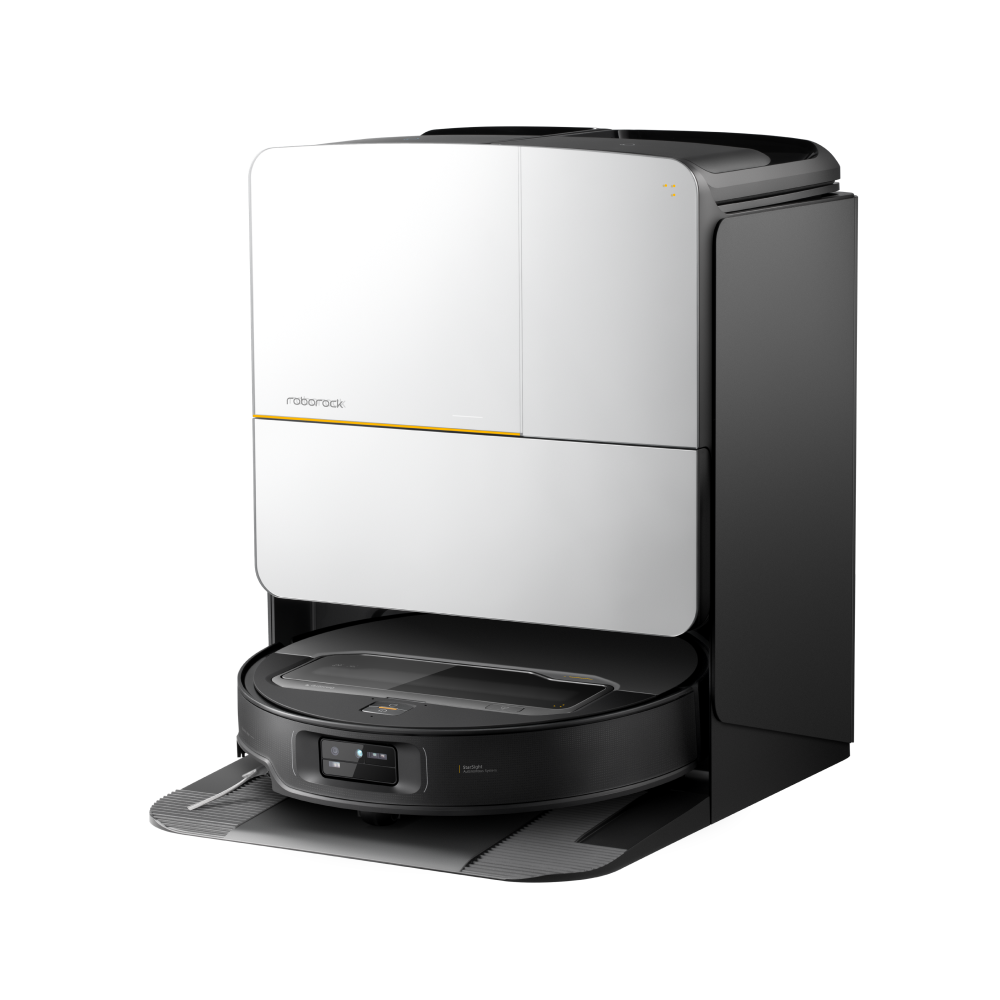
\includegraphics[width=\linewidth]{saros-z70.png}\\[-0.2em]
{\small Saros Z70}
\end{minipage}\hfill
\begin{minipage}[t]{0.30\textwidth}
\centering
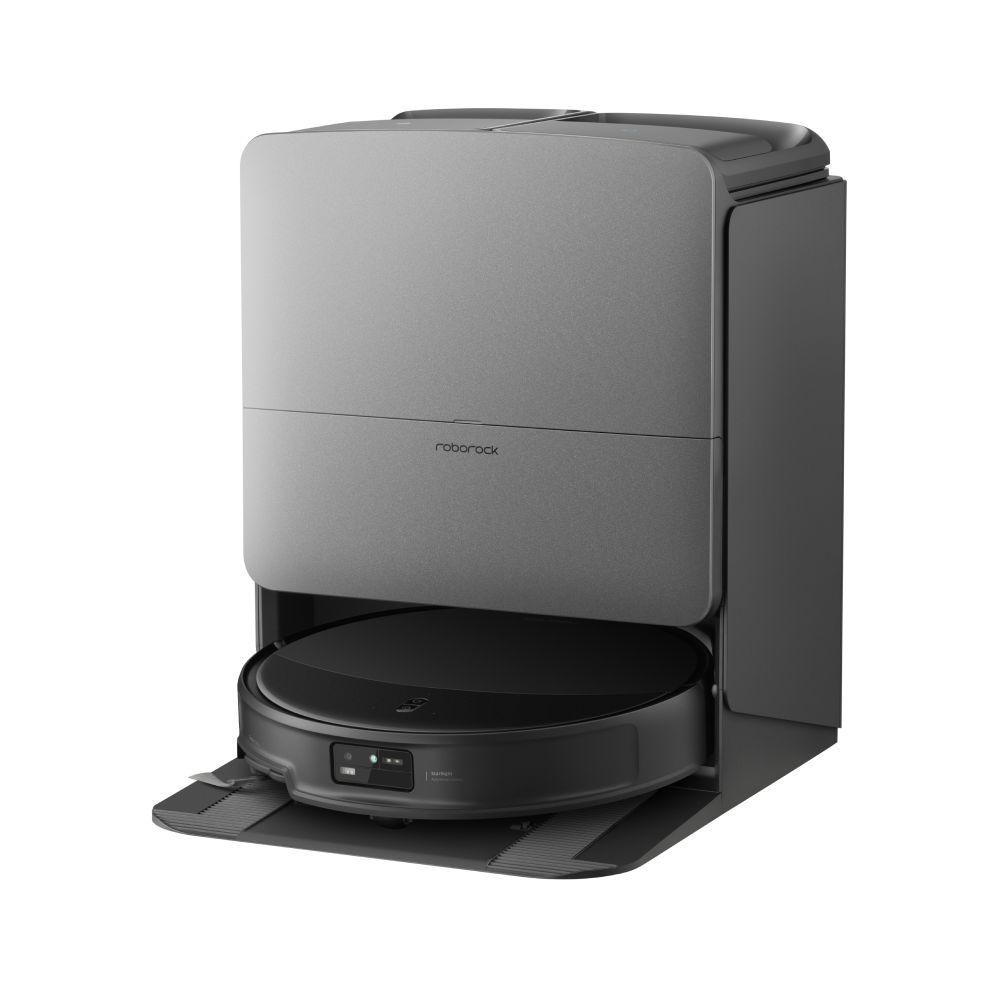
\includegraphics[width=\linewidth]{saros-20.png}\\[-0.2em]
{\small Saros 20}
\end{minipage}\hfill
\begin{minipage}[t]{0.30\textwidth}
\centering
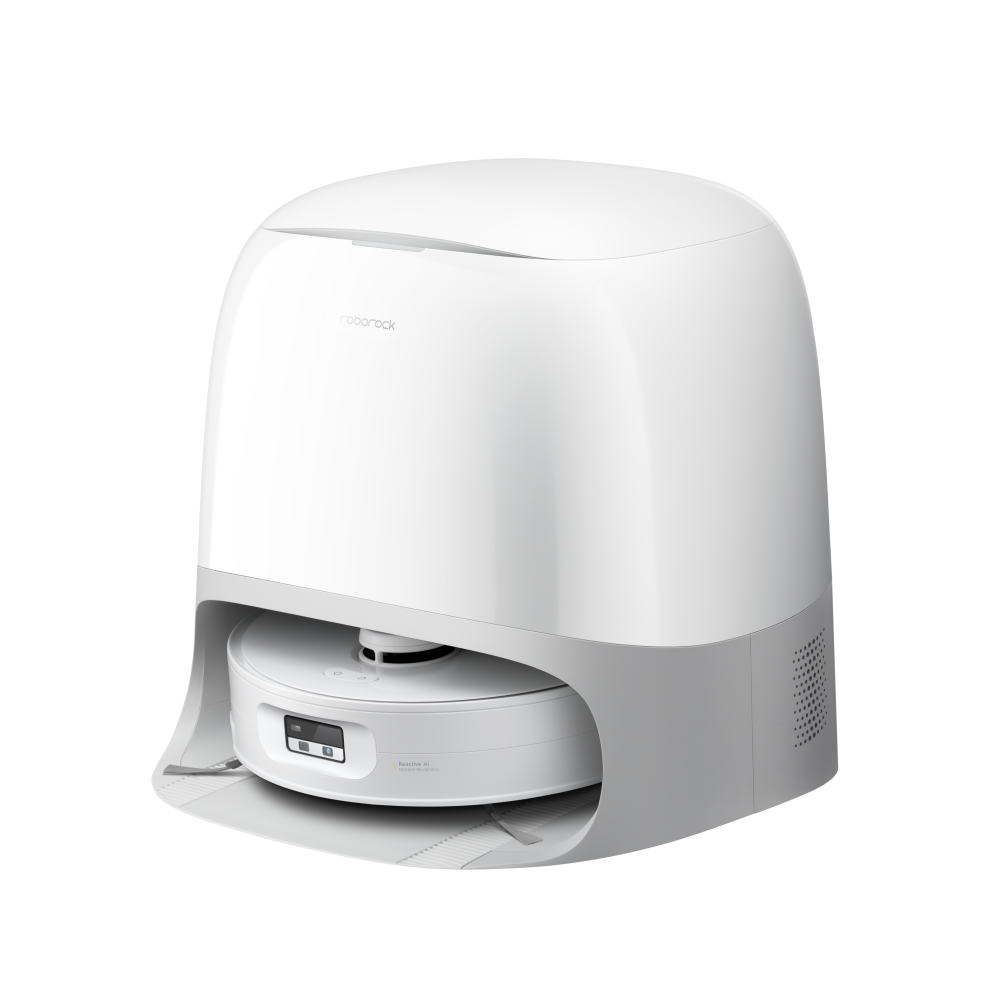
\includegraphics[width=\linewidth]{qrevo-curv-2-flow.png}\\[-0.2em]
{\small Qrevo Curv 2 Flow}
\end{minipage}

\vspace{0.7em}

\begin{minipage}[t]{0.30\textwidth}
\centering
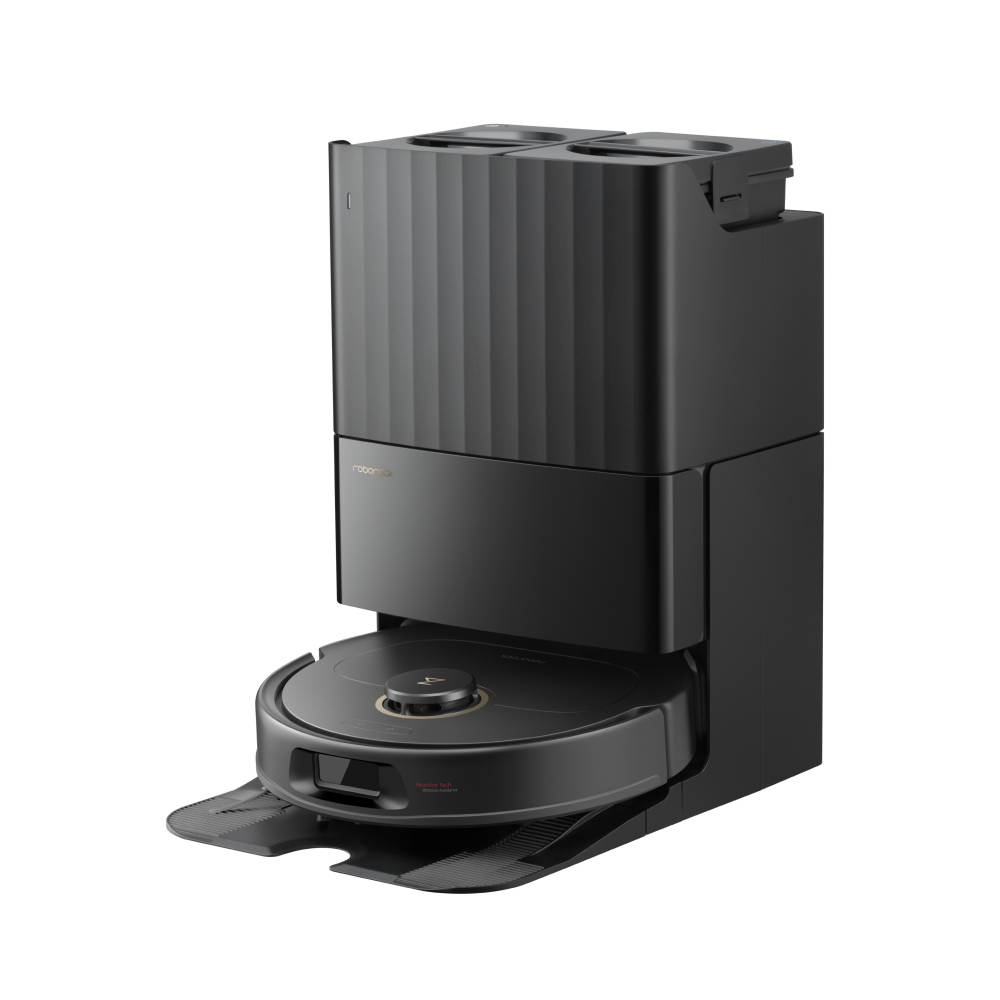
\includegraphics[width=\linewidth]{qrevo-series.png}\\[-0.2em]
{\small Qrevo Series}
\end{minipage}\hfill
\begin{minipage}[t]{0.30\textwidth}
\centering
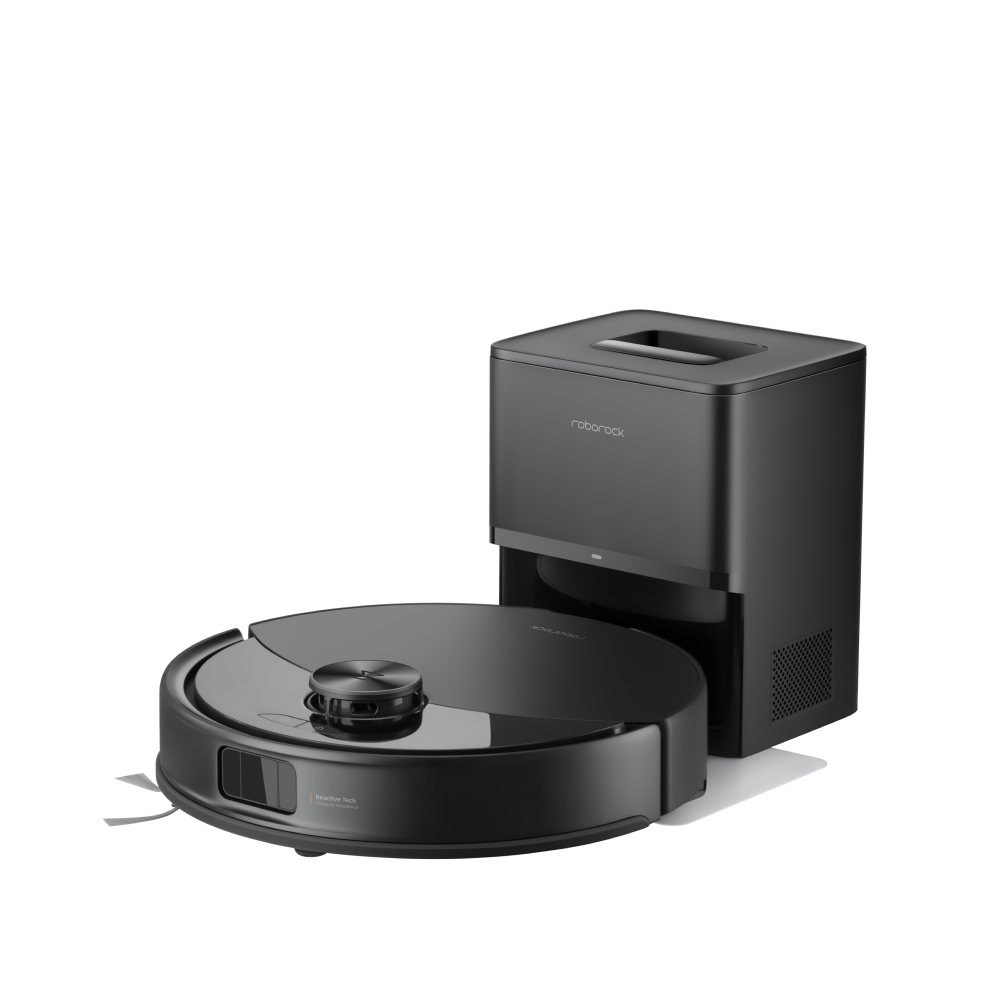
\includegraphics[width=\linewidth]{q10-series.png}\\[-0.2em]
{\small Q10 Series}
\end{minipage}\hfill
\begin{minipage}[t]{0.30\textwidth}
\centering
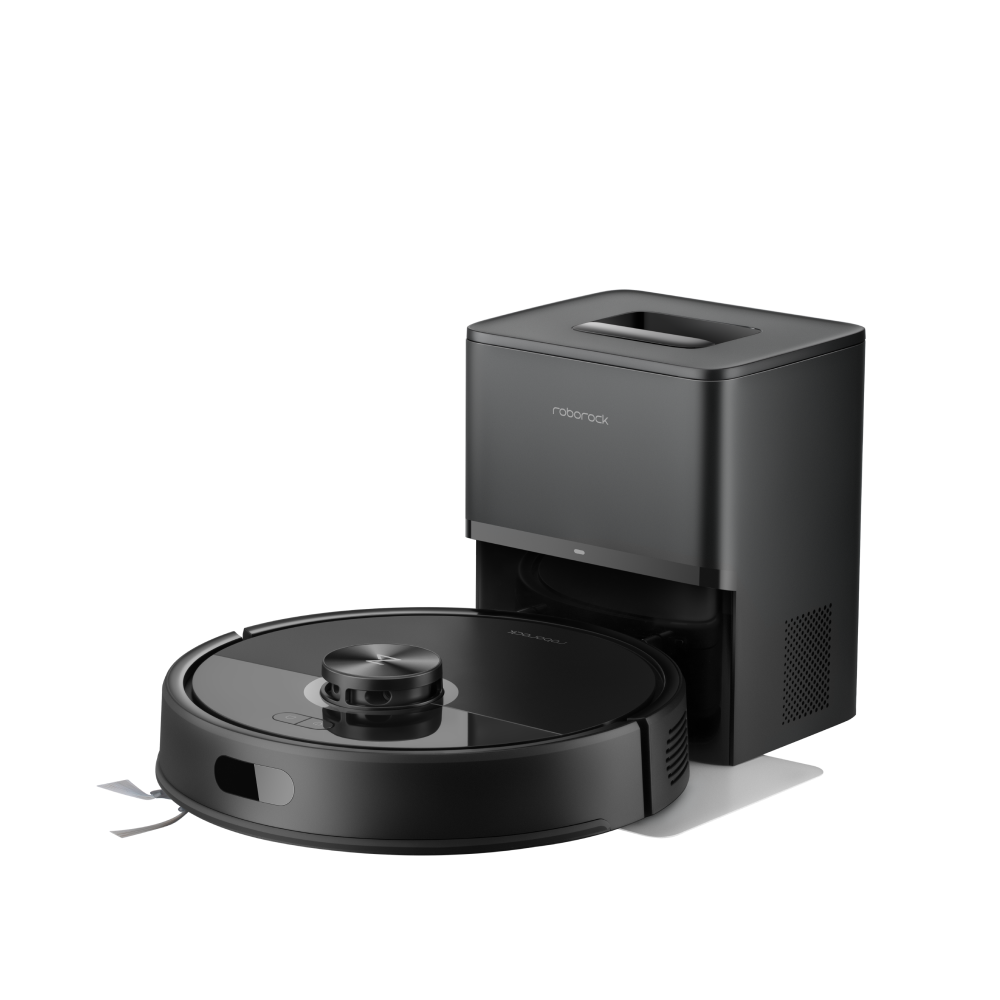
\includegraphics[width=\linewidth]{q7-series.png}\\[-0.2em]
{\small Q7 Series}
\end{minipage}
\caption{石头科技主要扫地机器人产品矩阵（图片来源：Roborock US Official Store与Roborock Global Official Store）}
\label{fig:roborock-product-matrix}
\end{figure}

本研究以扫地机器人为对象。ITC的HS6产品组850811用于筛选市场，中国海关85081110数据用于校准出口产品结构，企业年报和终端零售资料进一步落实到扫地机产品与经营实践。分析由产品组机会逐步收束到重点市场和企业适配。\src{中华人民共和国海关总署，海关统计数据在线查询平台，\url{http://stats.customs.gov.cn/}；国际贸易中心（ITC），Trade Map，产品HS850811。}

\subsection{世界生产与消费概览}

石头科技2024年年报转引IDC数据：全球智能扫地机器人出货量为2,060.3万台，同比增长11.2\%；销售额为93.1亿美元，同比增长19.7\%。2025年年报转引的全球出货量升至2,412.4万台，同比增长17.1\%。全球需求继续扩张，能否转化为中国企业的增长，还取决于供给能力和目的国需求结构。\src{北京石头世纪科技股份有限公司，《2024年年度报告》，PDF第18页、印刷第17页；《2025年年度报告》，第19页。两份年报均转引IDC。}

RCEP市场的普及程度并不一致。开源证券转引欧睿的2024年扫地机渗透率图显示，日本为5.4\%，韩国为8.1\%，澳大利亚为12.9\%。这些差异表明，区域内同时存在首次购买和存量升级两类需求，具体市场及对应策略将在筛选后进一步判断。\src{开源证券，《公司深度报告：新业务大幅减亏+扫地机行业竞争缓和，2026年净利率迎来拐点》，封面日期2026年2月4日，第17页图21，转引欧睿，采用图中2024年柱形标签。}

\subsection{中国生产能力}

中国具备较完整的家电供应链和电子制造基础，中国扫地机器人企业由此形成产品开发和规模化供给的产业条件。石头科技把研发、品牌和产品定义置于供应链之上，其年报同时指出，国内清洁电器渗透率仍有提升空间，海外市场已经成为企业增长的重要方向；公司通过品牌建设、全价格段覆盖和精细化渠道运营拓展海外用户。\src{石头科技，《2025年年度报告》，第10、15--16页。}

生产组织也在向区域协同延伸。石头科技采用自建工厂与委外加工结合的方式，2024年第四季度启动越南代工并陆续发货，2025年新增马来西亚代工业务。中国的研发和产品定义能力由此与RCEP区域制造网络相连，为后续的交付、原产地安排和产能调度提供了基础。\src{北京石头世纪科技股份有限公司，《2025年年度报告》，第26页。}

\subsection{案例企业：石头科技}

本文以石头科技观察中国扫地机器人企业如何把产业供给能力转化为RCEP市场中的产品和品牌能力。企业主体为北京石头世纪科技股份有限公司，品牌名为Roborock。公司以智能扫地机器人为核心主营产品，业务覆盖设计、研发、生产和销售，产品技术集中在环境感知、路径规划、清扫与拖地执行、基站自维护及移动端控制等环节。\src{北京石头世纪科技股份有限公司，《2025年年度报告》，第13--16页。}

石头科技的主营集中度和海外经营基础使其具有案例代表性。2025年智能扫地机及配件收入151.73亿元，占主营业务收入的81.22\%；境外主营业务收入104.42亿元，占55.90\%。公司年报转引IDC的智能扫地机器人全球份额为27.0\%，全球销量份额排名第一。\src{北京石头世纪科技股份有限公司，《2025年年度报告》，第20、26、54页。两项收入占比分别按15,172,943,325/18,680,324,995和10,441,601,948/18,680,324,995计算；全球份额为年报转引IDC口径。}

产品演进、中国供应链和石头科技的海外经营共同构成供给基础。下一步需要从全球贸易流向中判断需求集中在哪里，并据此确定RCEP市场的比较范围。

\section{全球贸易概览}

\subsection{世界贸易特点}

本文采用ITC Trade Map、Market Access Map和Export Potential Map的数据。Trade Map覆盖2020--2025年，金额原始单位为千美元；EPM输出EPI潜力和基准出口额，金额为美元；Market Access Map记录目的国税则线、税率方案和非关税措施。贸易与潜力比较使用HS850811，关税按目的国细分税则线核对。\src{国际贸易中心（ITC），Trade Map（\url{https://www.trademap.org/}）、Export Potential Map（\url{https://exportpotential.intracen.org/}）及Market Access Map（\url{https://www.macmap.org/}）。}

Trade Map描述规模、增长和供应结构，Export Potential Map衡量出口潜力，Market Access Map核对准入条件。三类数据依次回答市场有多大、还有多少拓展空间，以及进入市场需要满足哪些条件。

\begin{table}[H]
\centering
\caption{ITC数据在本研究中的作用}
\label{tab:itcdata}
\small
\begin{tabular}{p{2.8cm}p{5.5cm}p{5.4cm}}
\toprule
工具 & 进入模型的字段 & 本文用途\\
\midrule
Trade Map & 2025年进口额、2020--2025年CAGR、中国供应份额与排名 & 衡量市场规模、增长及中国供应基础\\
Export Potential Map & EPI、基准出口额、未实现潜力及其比例 & 衡量未来可拓展空间\\
Market Access Map & 目的国税则线、MFN与优惠税率、NTM记录 & 比较准入条件，不纳入五指标评分\\
\bottomrule
\end{tabular}
\par\vspace{0.4em}
\begin{minipage}{0.92\textwidth}\small
资料来源：ITC Trade Map、Export Potential Map与Market Access Map。
\end{minipage}
\end{table}

\subsection{进口特点}

RCEP候选市场在规模和增长之间存在明显差异。2025年日本HS850811产品组进口额为7.594亿美元，韩国为7.391亿美元，澳大利亚为5.228亿美元；马来西亚和新西兰分别为6,421万美元和5,846万美元。日本的规模最大，2020--2025年进口复合增长率却为$-5.71\%$；韩国、澳大利亚和马来西亚分别为8.65\%、7.25\%和16.41\%，新西兰为2.32\%。候选市场由此呈现大规模需求、较快扩张和小市场补充空间等不同组合。\src{国际贸易中心（ITC），Trade Map，HS850811，2020--2025年；来源ID为TM-392、TM-410、TM-036、TM-458、TM-554的target\_import\_imports\_by\_supplier-VAL记录。}

\begin{figure}[H]
\centering
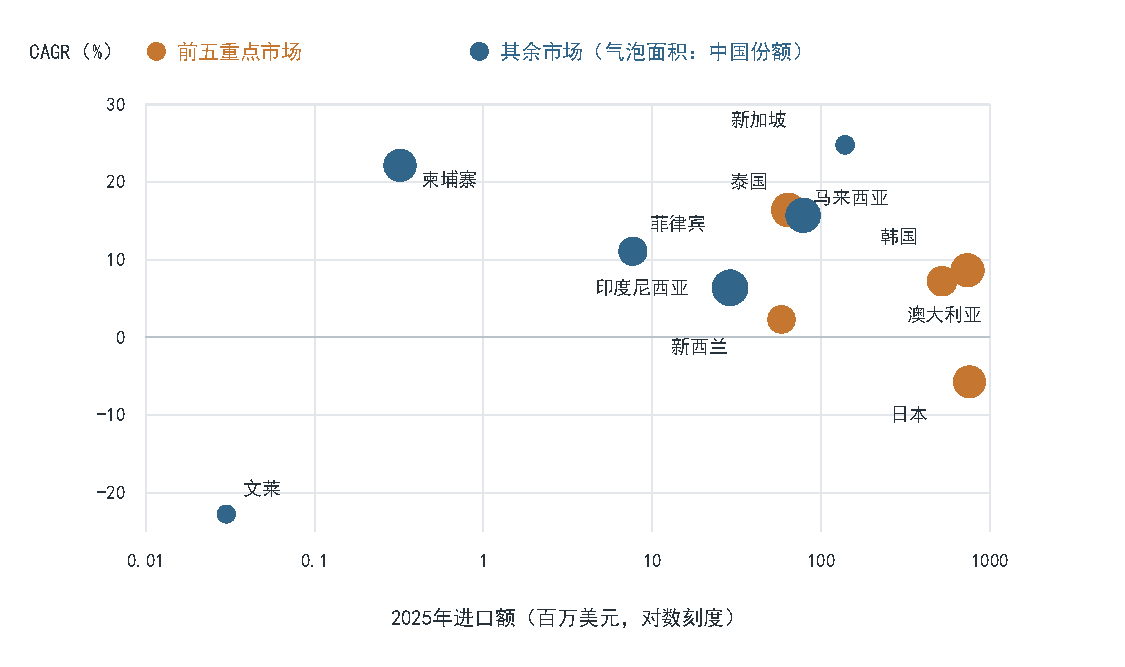
\includegraphics[width=0.92\textwidth]{market_size_growth.pdf}
\caption{RCEP候选市场的进口规模、增长率与中国供应份额}
\label{fig:sizegrowth}
\begin{minipage}{0.92\textwidth}\small
数据来源：ITC Trade Map，2020--2025年HS850811；绘制贸易字段完整的11个市场。横轴采用对数刻度，气泡面积表示2025年中国供应份额。
\end{minipage}
\end{figure}

图\ref{fig:sizegrowth}把规模与增长放在同一坐标中。柬埔寨和马来西亚的增速较高，2025年进口额分别为32.1万美元和6,421.3万美元；日本的规模优势则伴随五年负增长。规模决定需求基础，增长反映市场动能，两者与出口潜力共同构成下一阶段的筛选指标。\src{ITC Trade Map，HS850811；来源ID为TM-116、TM-458、TM-392的target\_import\_imports\_by\_supplier-VAL记录。}

\subsection{出口特点}

中国在五个重点市场均为该产品组的第一供应国，供应份额从新西兰的53.52\%至马来西亚的81.25\%不等。这一供给基础使中国企业能够把市场研究进一步推进到产品配置、品牌经营、渠道和售后环节，石头科技的适配分析也由此展开。\src{ITC Trade Map，HS850811，2025年按供应国进口数据；五国来源ID为TM-410、TM-036、TM-458、TM-554、TM-392的target\_import\_imports\_by\_supplier-VAL记录。}

全球贸易格局已经给出两点基础：RCEP需求规模与增长并不同步，中国则在重点市场拥有稳定供给位置。第三部分据此转向中国出口业绩，并考察石头科技承接这种产业优势时面临的经营约束。

\section{国家出口业绩}

\subsection{中国扫地机器人产品的世界市场表现}

按中国出口报告口径，2025年中国对韩国、澳大利亚、马来西亚、新西兰和日本出口HS850811的金额分别为3.803亿、2.351亿、6,888万、2,056万和4.627亿美元；按进口国报告口径，五国自中国进口额分别为5.798亿、3.246亿、5,218万、3,129万和5.502亿美元。后文以进口国报告值计算当地供应份额，中国出口报告值用于观察出口规模。\src{ITC Trade Map，HS850811，2025年；字段china\_direct\_exports\_usd\_thousand与imports\_from\_china\_usd\_thousand。五国来源ID为TM-410、TM-036、TM-458、TM-554、TM-392的china\_exports\_bilateral-VAL及target\_import\_imports\_by\_supplier-VAL记录。}

海关数据进一步显示，同一HS6范围下，各国的出口产品结构并不相同。2026年1--8月，85081110占850811的出口金额比重在韩国与澳大利亚超过一半，马来西亚与新西兰约为三分之一，日本约为四分之一。宽范围排名提供筛选起点，小范围结构则决定后续应把多少研究重点放在扫地机上。

\begin{table}[H]
\centering
\caption{2026年1--8月中国对重点市场两个税号范围的出口额}
\label{tab:customscompare}
\small
\begin{tabular}{lrrr}
\toprule
市场 & HS850811 & HS85081110 & 小范围金额占比\\
 & 亿元人民币 & 亿元人民币 & \%\\
\midrule
日本 & 18.85 & 4.68 & 24.85\\
韩国 & 18.13 & 9.65 & 53.22\\
澳大利亚 & 17.14 & 10.61 & 61.88\\
马来西亚 & 3.00 & 1.03 & 34.34\\
新西兰 & 1.27 & 0.48 & 37.53\\
美国（参照） & 42.30 & 18.07 & 42.72\\
\bottomrule
\end{tabular}
\par\vspace{0.4em}
\begin{minipage}{0.96\textwidth}\small
数据来源：中国海关2026年1--8月用户下载数据；占比按人民币出口金额计算。\src{中华人民共和国海关总署，海关统计数据在线查询平台，\url{http://stats.customs.gov.cn/}。}
\end{minipage}
\end{table}

\subsection{产品国际竞争力}

中国家电供应链、电子制造和规模化生产构成扫地机器人出口的产业基础。在企业层面，石头科技把这一基础转化为感知、决策、执行、基站自维护和移动端控制能力，并形成覆盖不同价格带的产品矩阵。\src{石头科技，《2025年年度报告》，第13--17页。}

增长与盈利的变化并不同步。Wind财务摘要显示，2023--2025年营业收入从86.54亿元增至186.95亿元，归母净利润从20.51亿元降至13.63亿元，经营现金净流量从21.86亿元降至7.74亿元；销售毛利率由55.13\%降至42.35\%，销售净利率由23.70\%降至7.29\%。2025年年报将境外毛利率下降与关税、运费及售后投入增加联系起来。这组变化更接近扩张期的成本消化压力，五国开拓要同时检查渠道占款和售价能否覆盖服务成本。\src{Wind，《石头科技[688169.SH]财务摘要》，2023--2025年合并报表，营业总收入、归属母公司股东的净利润、经营活动现金净流量、销售毛利率和销售净利率，原表单元格B5--D5、B14--D14、B40--D40、B57--D58；数值与《2025年年度报告》第10页逐项核对；经营原因见该年报第53--55页。}

\begin{figure}[H]
\centering
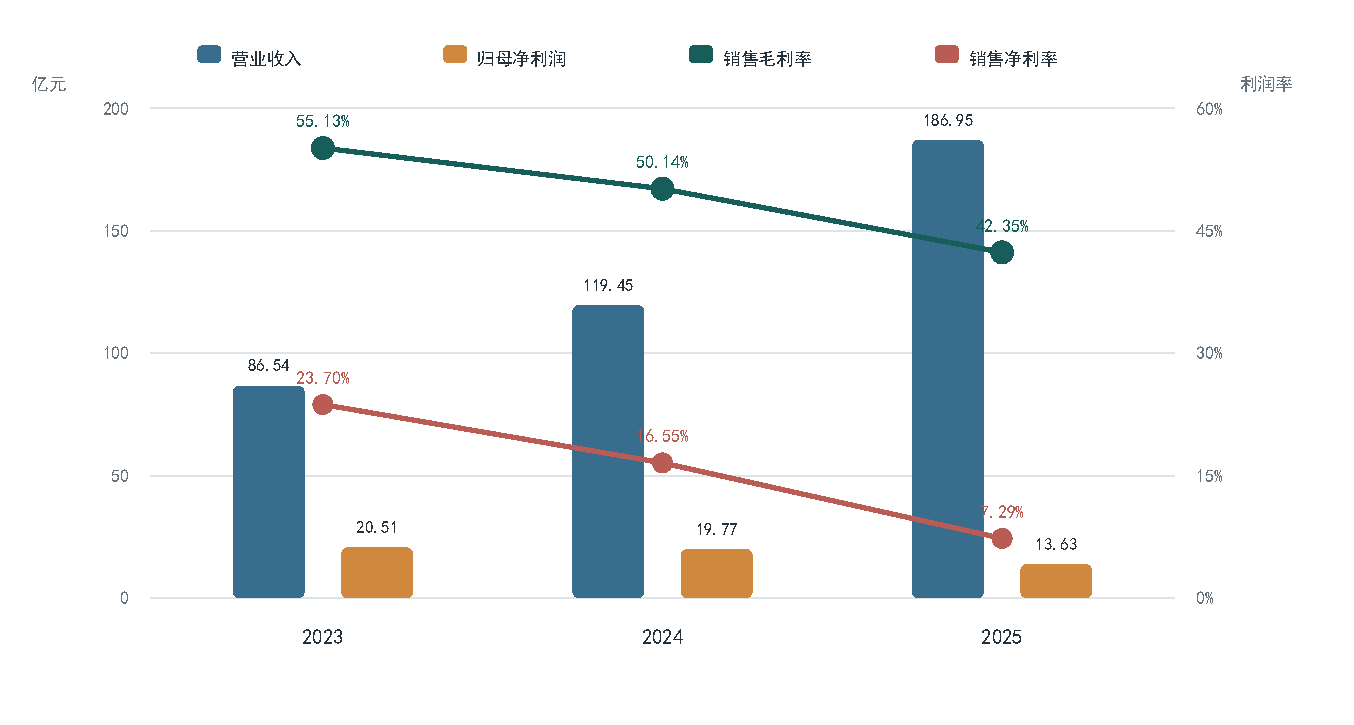
\includegraphics[width=\textwidth]{company_financial_trend.pdf}
\caption{石头科技收入、利润与经营现金净流量（2023--2025年）}
\label{fig:companyfinance}
\begin{minipage}{0.96\textwidth}\small
数据来源：Wind财务摘要，按合并报表口径计算；年报原表核对。两图均为亿元人民币，横轴尺度不同。\src{Wind财务摘要，北京石头世纪科技股份有限公司，《2025年年度报告》，第10页。}
\end{minipage}
\end{figure}

产品结构进一步说明了这一变化。2025年公司智能扫地机销售561.90万台，同比增长62.90\%，智能扫地机及配件收入增长39.86\%，该产品毛利率降至43.29\%。销量增长快于收入，扩展价格段时需要把产品组合与盈利能力一并纳入市场判断。\src{北京石头世纪科技股份有限公司，《2025年年度报告》，第54--55页，主营业务分产品情况及产销量情况分析表。销量原值5,618,978台，智能扫地机及配件收入同比39.86\%。}

中国扫地机器人企业也在持续改进成本管理。开源证券认为，科沃斯通过提高零部件自供比例和调整供应商压缩物料成本，清晰的滚筒卖点也降低了营销转化负担；报告据此解释其2025年下半年较好的盈利表现。这一行业经验对石头的启示是：功能增量、用户感知和供应链降本需要落实到同一型号，新增配置才有可能转化为稳定毛利。\src{开源证券，《公司深度报告：新业务大幅减亏+扫地机行业竞争缓和，2026年净利率迎来拐点》，2026年2月4日，第6页；《降本提效叠加竞争格局改善，扫地机龙头有望迎来业绩收获期》，2026年9月6日，第9页。}

% TODO[WIND-PRODUCT]: 补充五国分市场整机销量、整机收入和ASP；不得用“整机及配件收入/整机销量”代替整机ASP。

\subsection{关税与市场准入条件}

Market Access Map的2026年记录显示，日本、澳大利亚和新西兰相关税则线的MFN税率为0\%；韩国机器人税则线的MFN为8\%、RCEP对华税率为5.30\%，另列对华优惠税率0\%；马来西亚MFN为20\%、RCEP方案为18.20\%，另列对华优惠税率0\%。日韩澳新五国的准入成本由此分成零MFN税率和多方案择优两类。关税不进入市场吸引力评分，其对到岸成本的影响在第六部分展开。\src{ITC Market Access Map，税率年份2026，HS Rev.2022；来源ID为MACMAP-392-DUTY-850811010及850811090、MACMAP-036-DUTY-85081100、MACMAP-554-DUTY-85081100、MACMAP-410-DUTY-8508111000、MACMAP-458-DUTY-8508110000。}

中国的供给位置、石头的产品能力和扩张期成本约束已经明确。以下先筛选市场，第六部分再把原产资格、认证和通关要求并入分国建议。

\section{市场筛选}

\subsection{产品口径与前五市场选择的稳健性检验}
\label{sec:hsrobustness}

ITC以六位产品组HS850811建模，中国海关八位编码HS85081110可以进一步观察扫地机相关出口结构。本研究以2026年1--8月出口金额占比检验产品结构差异对重点市场选择的影响，样本与下文综合排序一致，均为数据完整的11个市场。

对市场$i$，先汇总各注册地和贸易方式的人民币出口额，再计算

\begin{equation}
s_i=\frac{X_{i,85081110}}{X_{i,850811}},
\label{eq:hsshare}
\end{equation}

其中$X$为同期出口金额，$s_i$为金额占比。表\ref{tab:customscompare}中，韩国、澳大利亚、马来西亚、新西兰和日本的占比分别为53.22\%、61.88\%、34.34\%、37.53\%和24.85\%。计算使用原始整数金额，展示时才舍入。\src{中华人民共和国海关总署，海关统计数据在线查询平台，\url{http://stats.customs.gov.cn/}；用户提供的2026年1--8月导出文件和六位表未提供数量字段，故使用两表共有的人民币金额。前五国占比对应事实编号S-KOR、S-AUS、S-MYS、S-NZL、S-JPN。}

检验采用两类情景。第一类把占比用于金额指标的代理调整，设$M_i$为进口规模、$U_i$为未实现潜力金额：

\begin{equation}
\begin{aligned}
\text{情景A：}\quad &(M_i',U_i')=(M_i,U_i s_i^{\alpha}),\\
\text{情景B：}\quad &(M_i',U_i')=(M_i s_i^{\alpha},U_i s_i^{\alpha}),
\qquad \alpha\in\{0.25,0.50,1.00\}.
\end{aligned}
\label{eq:hsamountadjustment}
\end{equation}

每个情景均从调整后的金额出发，重新执行下文的对数变换、极差标准化和原权重TOPSIS；增长率、中国供应份额及未实现潜力比例保持不变。八位占比在这里作为进口规模或潜力金额的缩放参数，用于观察六位模型的排名稳定性。

第二类把$s_i$作为第六项正向指标，先做极差标准化，再赋予5\%、10\%和20\%权重，原五项权重同比例缩减：

\begin{equation}
z_{i6}=\frac{s_i-\min_i s_i}{\max_i s_i-\min_i s_i},\qquad
w_k'=(1-\lambda)w_k\ (k=1,\ldots,5),\quad w_6'=\lambda.
\label{eq:hsshareweights}
\end{equation}

其中$\lambda\in\{0.05,0.10,0.20\}$，$w_k$沿用表\ref{tab:weights}。这一情景衡量在市场吸引力之外增加产品结构偏好后，筛选结果是否稳定。\src{本研究，HS85081110占比对ITC排名的验证，运行编号20261010-HS85081110-share-ITC-ranking-verification；原模型编号20261010T153053-CHN-HS850811-RCEP-TOPSIS。}

设$R_i$和$R_i'$为原模型与情景模型的名次，名次越小越靠前。使用Pearson名次相关、Spearman秩相关和Kendall秩相关比较整体次序：

\begin{equation}
\begin{aligned}
r_R&=\frac{\sum_i(R_i-\bar R)(R_i'-\bar R')}
{\sqrt{\sum_i(R_i-\bar R)^2\sum_i(R_i'-\bar R')^2}},\\
\rho&=1-\frac{6\sum_i(R_i-R_i')^2}{n(n^2-1)},\qquad
\tau=\frac{N_c-N_d}{\binom{n}{2}}.
\end{aligned}
\label{eq:hsrankagreement}
\end{equation}

其中$n=11$，$N_c$、$N_d$分别为两组排名中的一致国家对和逆序国家对。本组情景没有并列名次，故$r_R=\rho$，表中合并列示。再以最大名次变化$\Delta_{\max}$和前五重合度$H_5$检验选择结果：

\begin{equation}
\Delta_{\max}=\max_i|R_i-R_i'|,\qquad
H_5=\frac{|T_5\cap T_5'|}{5},
\label{eq:hstopfiveoverlap}
\end{equation}

其中$T_5$、$T_5'$分别为原模型与情景模型的前五市场集合。

\begin{table}[H]
\centering
\caption{产品结构调整下前五市场的稳定性}
\label{tab:hsrobustness}
\small
\setlength{\tabcolsep}{5pt}
\begin{tabular}{>{\raggedright\arraybackslash}p{6.4cm}rrrr}
\toprule
情景 & $r_R=\rho$ & $\tau$ & $\Delta_{\max}$ & $H_5$\\
\midrule
仅调整未实现潜力金额，$\alpha=0.25,0.50,1.00$ & 1.0000 & 1.0000 & 0 & 100\%\\
同时调整规模与潜力金额，$\alpha=0.25,0.50,1.00$ & 1.0000 & 1.0000 & 0 & 100\%\\
占比作为第六指标，$\lambda=5\%$ & 1.0000 & 1.0000 & 0 & 100\%\\
占比作为第六指标，$\lambda=10\%$ & 1.0000 & 1.0000 & 0 & 100\%\\
占比作为第六指标，$\lambda=20\%$ & 0.9818 & 0.9273 & 1 & 100\%\\
\bottomrule
\end{tabular}
\par\vspace{0.4em}
\begin{minipage}{0.95\textwidth}\small
数据来源：本研究据海关出口金额及ITC原模型计算；前两行分别汇总三个参数情景，各项排名统计量在三个情景中相同。
\end{minipage}
\end{table}

表\ref{tab:hsrobustness}显示，两类金额调整下11国排序均未改变；新增占比指标的权重为5\%或10\%时，排序也完全一致。权重提高到20\%后，仅两组相邻市场交换名次，最大变化为一位：新西兰由第四升至第三，马来西亚由第三降至第四；印度尼西亚与泰国在第六、第七位互换。韩国、澳大利亚、马来西亚、新西兰和日本始终保留在前五。\src{本研究，运行编号20261010-HS85081110-share-ITC-ranking-verification，事实编号V-020及V-021。}

上述情景的前五市场始终不变，六位口径足以支撑初步筛选。后文保留ITC五指标模型和五国研究范围，再用八位出口结构、终端产品和渠道证据细化各国的开拓任务。

\subsection{市场筛选思路与指标体系}

市场筛选分为两步：先比较产品和产业层面的外部吸引力，再结合石头科技的产品、渠道和经营基础判断适配程度。前一步确定研究范围，后一步形成分国问题。

\subsubsection{ITC出口潜力框架}

ITC出口潜力指标把出口国供给能力、目标市场需求和双边贸易便利度结合起来。对出口国$i$、目标市场$j$和产品$k$，基本关系为

\begin{equation}
EPI_{ijk}=Supply_{ik}\times Ease_{ij}\times Demand_{ijk}.
\end{equation}

本研究采用Export Potential Map公布的EPI。未实现潜力按每个“中国—目的国—HS850811”组合计算，其中$ActualExports$取EPM的基准出口额：

\begin{equation}
Untapped_{ijk}=\max\left(EPI_{ijk}-ActualExports_{ijk},0\right).
\end{equation}

EPI综合供给、需求和双边贸易条件，未实现比例为$Untapped/EPI$。它与贸易规模共同确定市场机会，渠道费用、认证、售后和品牌基础则进入第二阶段的企业适配分析。\src{ITC Export Potential Map，中国向RCEP成员国出口HS850811；逐国来源ID为EPM加三位国家代码。未实现额及比例据官方潜在额与基准出口额计算。}

\subsubsection{指标、变换与权重}

候选范围包括东盟十国、澳大利亚、新西兰、日本和韩国。综合排序使用进口规模、增长和中国份额均完整的11个市场；老挝、缅甸和越南列入机会观察。金额指标采用$\ln(1+x)$平衡不同市场的数量级，增长率、份额和潜力比例直接做极差标准化。正向指标的标准化公式为

\begin{equation}
z_{ij}=\frac{x_{ij}-\min(x_j)}{\max(x_j)-\min(x_j)}.
\end{equation}

\begin{table}[H]
\centering
\caption{市场吸引力模型的指标与战略权重}
\label{tab:weights}
\small
\begin{tabular}{p{3.2cm}p{3.4cm}p{3.2cm}r}
\toprule
指标 & 原始字段 & 变换 & 权重\\
\midrule
市场规模 & 2025年进口额 & $\ln(1+x)$后Min--Max & 0.30\\
市场增长 & 2020--2025年CAGR & Min--Max & 0.10\\
中国竞争位置 & 2025年中国供应份额 & Min--Max & 0.10\\
未实现潜力金额 & EPI减基准出口额 & $\ln(1+x)$后Min--Max & 0.30\\
未实现潜力比例 & 未实现潜力除以EPI & Min--Max & 0.20\\
\bottomrule
\end{tabular}
\par\vspace{0.4em}
\begin{minipage}{0.92\textwidth}\small
资料来源：本研究依据ITC数据计算；沿用原研究设定的战略权重。
\end{minipage}
\end{table}

进口规模和未实现潜力各占30\%，分别衡量现有需求和可拓展空间；潜力比例占20\%，增长和中国份额各占10\%。权重突出规模与新增空间，稳健性比较使用等权、熵权和5,000组随机扰动结果。\src{本研究据ITC数据计算；模型运行编号20261010T153053-CHN-HS850811-RCEP-TOPSIS。}

\subsubsection{TOPSIS排序过程}

标准化矩阵乘以权重得到$v_{ij}=w_jz_{ij}$。每个市场到正理想解和负理想解的距离分别为

\begin{equation}
D_i^+=\sqrt{\sum_j(v_{ij}-v_j^+)^2},\qquad
D_i^-=\sqrt{\sum_j(v_{ij}-v_j^-)^2},
\end{equation}

最终贴近度为

\begin{equation}
C_i=\frac{D_i^-}{D_i^++D_i^-}.
\end{equation}

$C_i$越高，市场在当前指标和权重下越接近理想组合。

\subsection{第一阶段：市场吸引力筛选}

\begin{figure}[H]
\centering
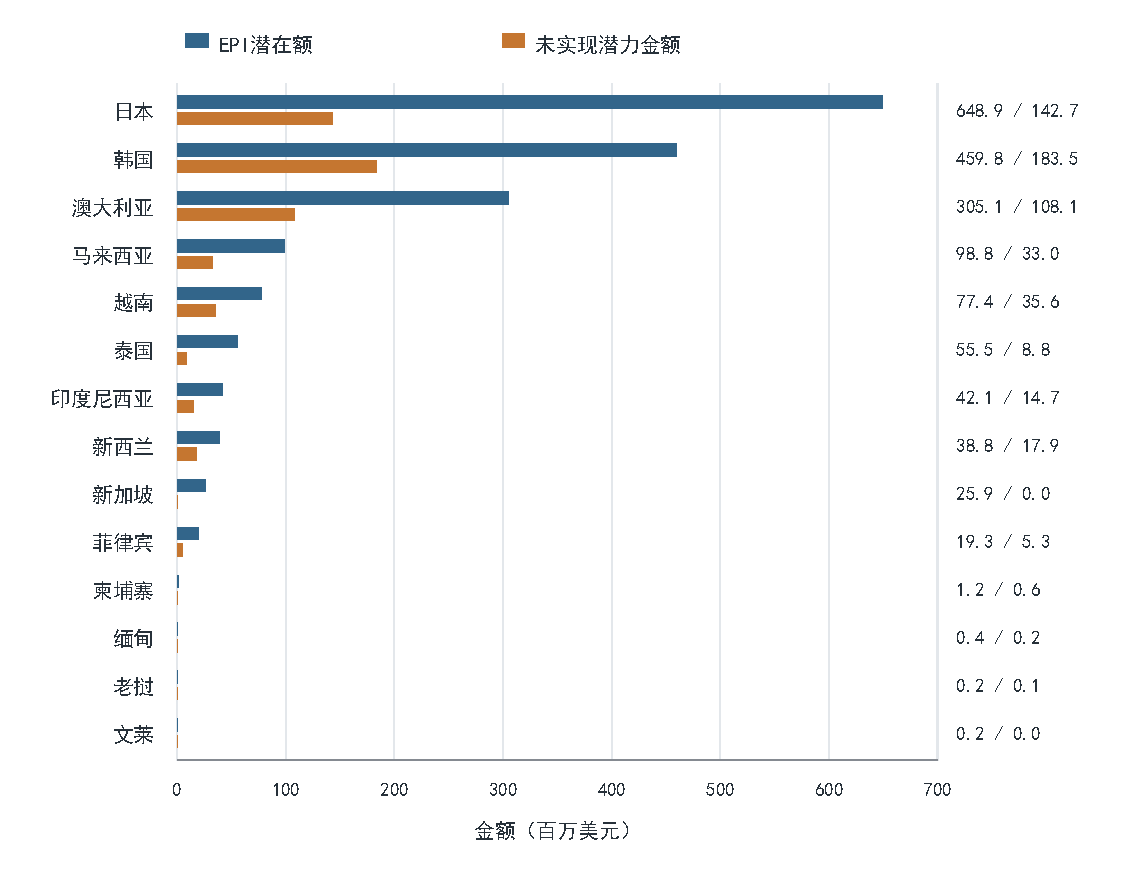
\includegraphics[width=0.92\textwidth]{epi_untapped.pdf}
\caption{中国向RCEP候选市场出口HS850811的EPI与未实现潜力}
\label{fig:epi}
\begin{minipage}{0.92\textwidth}\small
数据来源：ITC Export Potential Map，出口国为中国，产品组HS850811未实现潜力逐国计算。
\end{minipage}
\end{figure}

图\ref{fig:epi}显示，日本、韩国和澳大利亚的EPI绝对值较高，未实现潜力金额则由韩国领先。马来西亚和新西兰的金额较小，但相对各自EPI仍有补充空间。越南保留EPM结果，因缺少2025年进口数据而列入机会观察名单，不进入综合排名。

\begin{table}[H]
\centering
\caption{前五市场的贸易与潜力指标}
\label{tab:top3}
\small
\setlength{\tabcolsep}{4pt}
\begin{tabular}{lrrrrrrr}
\toprule
市场 & 进口额 & 五年CAGR & 中国份额 & EPI潜力 & 未实现额 & 潜力占比 & 得分\\
 & 百万美元 & \% & \% & 百万美元 & 百万美元 & \% & \\
\midrule
韩国 & 739.15 & 8.65 & 78.44 & 459.78 & 183.52 & 39.92 & 0.8963\\
澳大利亚 & 522.80 & 7.25 & 62.09 & 305.05 & 108.09 & 35.43 & 0.8462\\
马来西亚 & 64.21 & 16.41 & 81.25 & 98.77 & 32.98 & 33.39 & 0.7936\\
新西兰 & 58.46 & 2.32 & 53.52 & 38.77 & 17.94 & 46.29 & 0.7808\\
日本 & 759.36 & -5.71 & 72.46 & 648.92 & 142.67 & 21.99 & 0.7703\\
\bottomrule
\end{tabular}
\par\vspace{0.4em}
\begin{minipage}{0.92\textwidth}\small
数据来源：ITC Trade Map的2025年进口额、供应份额及2020--2025年增长，以及Export Potential Map；金额仅为展示换算为百万美元，计算仍用原单位。\src{来源ID TM-410、TM-036、TM-458、TM-554、TM-392对应进口记录及EPM-410、EPM-036、EPM-458、EPM-554、EPM-392。}
\end{minipage}
\end{table}

\begin{figure}[H]
\centering
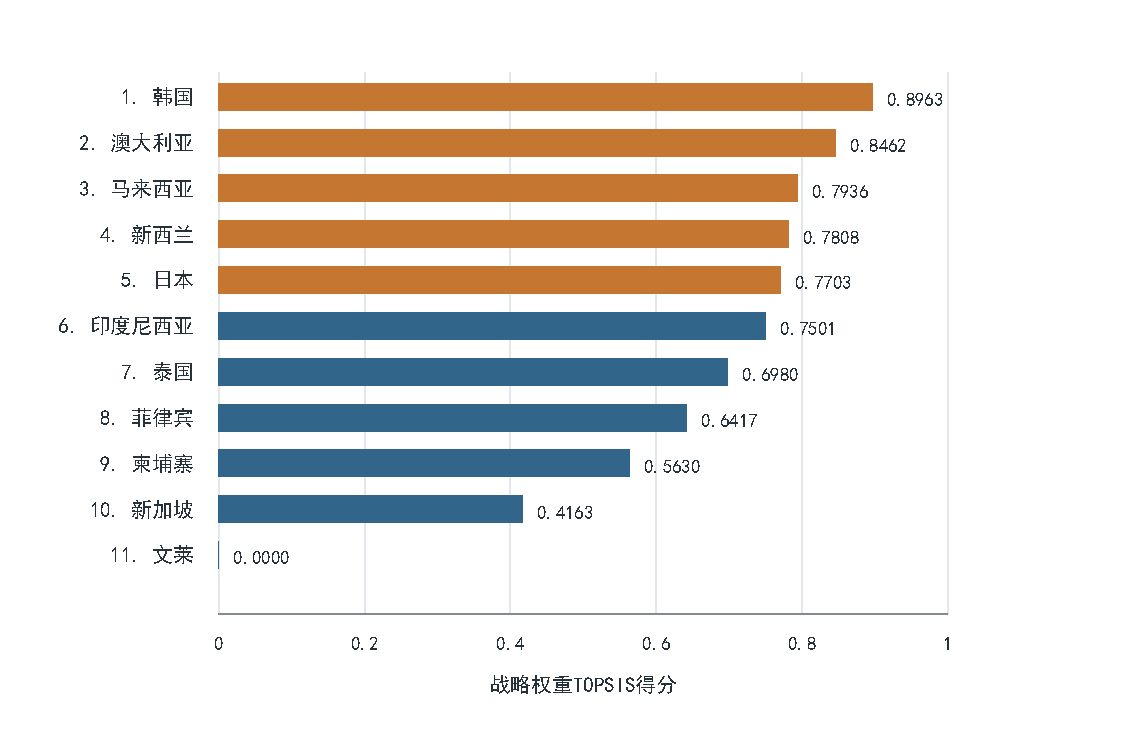
\includegraphics[width=0.90\textwidth]{market_score.pdf}
\caption{战略权重TOPSIS市场吸引力得分}
\label{fig:score}
\begin{minipage}{0.90\textwidth}\small
数据来源：既有HS850811模型；按表\ref{tab:weights}计算。橙色为前五市场，关税与NTM不进入评分。
\end{minipage}
\end{figure}

战略权重下，韩国、澳大利亚、马来西亚、新西兰和日本依次位列前五，得分见表\ref{tab:top3}。韩国与澳大利亚兼有较大规模和正增长，马来西亚突出增长，新西兰突出相对潜力，日本保留最大的需求池。排序由此转化为五项研究任务：增长承接、常态经营、品牌覆盖、细分供货和存量升级。\src{本研究战略权重TOPSIS结果；模型运行编号20261010T153053-CHN-HS850811-RCEP-TOPSIS。}

韩国的进口额接近日本，五年增长为正，未实现潜力金额在候选市场中最高。EPM基准出口额2.763亿美元相当于潜在额的60.08\%，使大市场仍保有相对空间；中国供应份额由44.88\%升至78.44\%，供货联系也在增强。后续重点是品牌竞争力，以及代理渠道承接新增需求的能力。\src{ITC Trade Map与Export Potential Map，来源ID为TM-410-target\_import\_imports\_by\_supplier-VAL、EPM-410。2020年中国份额按219113/488183计算，实现比例按276250466.67/459775312.98计算。}

澳大利亚进口额由2020年的3.685亿美元升至2025年的5.228亿美元，中国来源增长更快，份额由35.09\%升至62.09\%。未实现潜力占比35.43\%，规模与新增空间共同支撑第二名。马来西亚来源仍占22.82\%，后续需区分品牌竞争与生产来源变化，并结合已有促销和渠道证据研究常态销售。\src{ITC Trade Map与Export Potential Map，来源ID为TM-036-target\_import\_imports\_by\_supplier-VAL、EPM-036。2020年中国份额按129289/368488计算。}

马来西亚16.41\%的增速来自进口额由3,003万美元增至6,421万美元，起点较小，规模仍远小于韩国和澳大利亚。中国供应份额81.25\%低于2020年的87.74\%，供货增加并未带来份额提升。6,579万美元基准额与9,877万美元EPI的差额形成33.39\%的未实现比例。后续要辨认增长集中的产品与价格带，检验石头科技扩大品牌覆盖的条件。\src{ITC Trade Map与Export Potential Map，来源ID为TM-458-target\_import\_imports\_by\_supplier-VAL、EPM-458。2020年中国份额按26352/30034计算。}

新西兰规模小、增长低，潜力占比却较高。基准出口额2,082万美元相当于3,877万美元潜在额的53.71\%，剩余比例46.29\%居五国首位，对应金额仅1,794万美元。中国供应份额由30.86\%升至53.52\%，总进口CAGR仅2.32\%，供货来源变化比需求扩张更突出。后续先验证细分用户与渠道容量，再形成销量判断。\src{ITC Trade Map与Export Potential Map，来源ID为TM-554-target\_import\_imports\_by\_supplier-VAL、EPM-554。2020年中国份额按16090/52133计算。}

日本未实现潜力占比较低，因为5.063亿美元基准出口额已占6.489亿美元潜在额的78.01\%，剩余21.99\%仍对应1.427亿美元。2020--2025年总进口由10.189亿美元降至7.594亿美元，自中国进口反由5.125亿美元升至5.502亿美元，收缩主要来自其他来源。日本的规模基础仍在，后续研究由新增规模转向扫地机的替代、升级和品牌经营。\src{ITC Trade Map与Export Potential Map，来源ID为TM-392-target\_import\_imports\_by\_supplier-VAL、EPM-392。实现比例按506251200/648919894.53计算；其他来源合计为世界进口额减自中国进口额。}

\subsubsection{敏感性检验}

等权与熵权下，马来西亚均升至第二，日本则分别降至第八和第七。马来西亚的名次随权重变化，但前五位置较稳定。5,000组随机权重中，韩国、澳大利亚、马来西亚、新西兰和日本进入前五的比例分别为100.00\%、99.76\%、99.88\%、80.44\%和65.26\%；印度尼西亚为44.78\%，可作为边界观察市场。前五集合较稳定，内部次序则留待经营证据进一步判断。\src{本研究依据既有模型的5,000组随机排名记录计算；前五频率按rank不大于5的次数除以5000统计。}

日本在剔除潜力比例指标时升至第三，金额不取对数时升至第二，说明其优势主要来自绝对规模。敏感性结果支持保留五国研究范围，并按不同指标优势继续分国分析。\src{本研究既有敏感性结果；日本leave\_out\_untapped\_ratio及amounts\_without\_log1p场景；模型运行编号20261010T153053-CHN-HS850811-RCEP-TOPSIS。}

\begin{figure}[H]
\centering
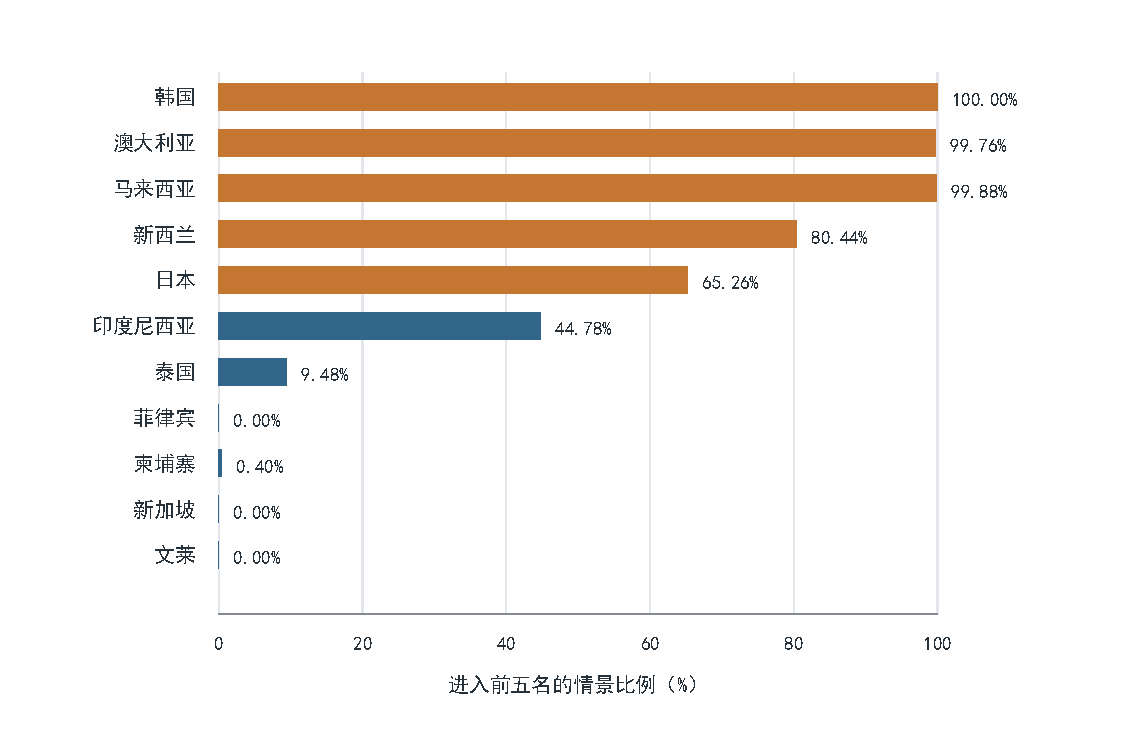
\includegraphics[width=0.90\textwidth]{ranking_sensitivity.pdf}
\caption{5,000组权重扰动情景下进入前五名的比例}
\label{fig:sensitivity}
\begin{minipage}{0.90\textwidth}\small
数据来源：既有模型的5,000组随机排名记录，权重沿用以战略权重为中心的Dirichlet分布。本图仅重新统计前五频率，未改变抽样。
% 历史随机种子850980保持不变，与本轮产品编码无关，另见图表provenance。
\end{minipage}
\end{figure}

\subsection{第二阶段：石头科技适配度}

\subsubsection{北美与欧洲的市场拓展路径}
石头科技在北美和欧洲市场的业务较为成熟，可以为五国开拓提供参考。

首先，美国的渠道扩展呈现由线上向线下推进的次序。2022年年报列示Amazon、Home Depot、Target等线上品牌店，2023年披露首次进入美国Target线下并覆盖180多家门店；2024年年报列示北美Target覆盖1,398家、Best Buy覆盖900家。2025年，公司继续依托Target、Costco和Home Depot扩展门店与SKU。石头先在线上积累品牌和用户，再借助连锁零售扩大触达，这一路径可为RCEP市场的渠道组合提供参照。\src{北京石头世纪科技股份有限公司，《2022年年度报告》，第12页；《2023年年度报告》，第15页；《2024年年度报告》，PDF第44页、印刷第43页；《2025年年度报告》，第23页。180多家为2023年美国Target门店；2024年1,398家及900家沿用年报“北美”区域口径。}

线下覆盖也会随零售商安排变化。2026年2月研报预计Best Buy渠道当年增量有限，9月研报又记录石头于第二季度重新入驻。渠道关系具有阶段性，五国开拓需要保留替代渠道，并分别跟踪谈判进度、陈列SKU和实际回款。\src{开源证券，2026年2月4日公司深度报告，第21页；《降本提效叠加竞争格局改善，扫地机龙头有望迎来业绩收获期》，2026年9月6日，第15页。}

欧洲同时推进平台经营与本土零售布局。2025年年报披露进入MediaMarkt、家乐福等零售系统；开源证券记录，石头于2024年4月进入法国Boulanger、Darty线下渠道。该券商2026年9月报告图16列示，第二季度石头在德国、法国亚马逊的份额分别为52.9\%、27.2\%。平台表现提供用户基础，本土零售承担体验与服务，两类渠道需要按国家进度协同。\src{北京石头世纪科技股份有限公司，《2025年年度报告》，第23页；开源证券，《公司深度报告：新业务大幅减亏+扫地机行业竞争缓和，2026年净利率迎来拐点》，封面日期2026年2月4日，第26页；《降本提效叠加竞争格局改善，扫地机龙头有望迎来业绩收获期》，封面日期2026年9月6日，第10页图16。}

欧洲门店采样显示，中国品牌在线上和线下形成了不同优势：石头线上份额较高，追觅线下份额略高。石头的经营特点是先围绕自有品牌持续经营平台用户，再增加本土零售触点。五国适配因而要同时考察产品吸引力和渠道转化能力。\src{开源证券，《降本提效叠加竞争格局改善，扫地机龙头有望迎来业绩收获期》，2026年9月6日，第10--14页；公司品牌与渠道经营依据见上述年报。}

\subsubsection{五国经营基础与适配重点}

第二阶段承接前五市场的筛选结果，比较石头已有经营基础、产品梯度和渠道条件。日韩已有海外公司，日本、澳大利亚列入前期布局，马来西亚已有品牌份额和代工证据；马来西亚与新西兰的零售资料分别用于检验价格梯度以及供货、服务条件。\src{北京石头世纪科技股份有限公司，《2022年年度报告》，第12页；《2025年年度报告》，第22、26页；开源证券，2026年2月4日公司深度报告，第28页正文、第29页图43，转引欧睿2024年马来西亚品牌份额。}

\begin{table}[H]
\centering
\caption{重点市场与石头科技已有经营基础的对应}
\label{tab:casefit}
\small
\begin{tabular}{p{1.9cm}p{4.7cm}p{6.6cm}}
\toprule
市场 & 已有证据 & 对后续研究的含义\\
\midrule
日本 & 已设海外公司；Kakaku采得20个Roborock产品条目 & 核对中高价位产品的配置差异、渠道报价与售后体验\\
韩国 & 已设海外公司；研报转引2024年石头份额30\%；Danawa一般购买样本20条 & 研究已有品牌基础如何与代理商经营和服务衔接\\
澳大利亚 & 已布局市场；研报转引2024年石头份额25\%；GetPrice样本7条 & 结合促销销量与零售供货，比较不同价位产品的持续销售能力\\
马来西亚 & 研报转引2024年石头份额8\%；PriceShop取得12个石头缓存产品页及新品报道；2025年新增当地代工 & 以多层级产品验证品牌触达与价格梯度，并衔接当地销售和售后\\
新西兰 & PriceSpy取得9个石头产品页，其中8个有合格新品报价，覆盖Q7B+、Qrevo与Saros系列 & 从逐型号供货、保修和维修条件判断细分经营空间\\
\bottomrule
\end{tabular}
\par\vspace{0.4em}
\begin{minipage}{0.96\textwidth}\small
资料来源：公司年报、开源证券与五国零售资料；各国产品页计数口径见表\ref{tab:retailsample}。\src{公司经营基础见上引年报；开源证券，2026年2月4日公司深度报告，第28页正文及第29页图43，转引欧睿；马来西亚事实编号RR26-0194、RR26-0169；PriceSpy与PriceShop产品资料。}
\end{minipage}
\end{table}

第二阶段据现有证据形成五项适配任务：日韩澳深化既有经营，马来西亚检验品牌覆盖，新西兰验证少量型号的持续供货与服务。

% TODO[WIND-STRATEGY]: 补充五国首次进入时间及管理层对分国资源安排的公开表述，优先补马来西亚和新西兰。
% TODO[WIND-COMPANY]: 补充五国同口径收入、利润、渠道覆盖和售后指标，再确定是否进行企业适配量化评分。

\subsection{市场选择结论}

第一阶段保留韩国、澳大利亚、马来西亚、新西兰和日本作为重点研究对象，印度尼西亚列入边界观察。第二阶段把前五名转化为分国问题。第五部分沿贸易绩效、竞争、季节性和价格比较五国，第六部分再以石头科技的既有能力回应这些问题。

\section{目标市场特性}

\subsection{目标市场的贸易绩效评估}

第4.1节表明，八位产品结构差异没有改变前五市场集合；表\ref{tab:top3}的规模、增长与潜力组合则决定了五国的研究方向。以下以扫地机终端销售、产品和渠道资料逐项检验这些机会。

贸易产品组之外，扫地机终端市场提供了另一层比较。开源证券转引欧睿数据，2024年韩国扫地机销售额为2.68亿美元，五年CAGR为15\%；澳大利亚为1.38亿美元，五年CAGR为7\%，两国当年同比增速分别为4\%和9\%。韩国的绝对规模与长期增长更强，澳大利亚当年增长更快；日本则结合产品层级与渠道资料观察替代和升级需求。\src{开源证券，2026年2月4日公司深度报告，第27页图37、图38及正文，转引欧睿；销售额与五年CAGR取该页明确列示值，2024年同比采用图题标注。}

同一研报图42列示马来西亚2024年扫地机销售额为0.20亿美元，同比增长10\%。终端规模小于韩国和澳大利亚，仍在扩张；产品研究应兼顾首次购买门槛与升级功能。\src{开源证券，2026年2月4日公司深度报告，第28页图42，转引欧睿；采用图表列示的0.20亿美元及10\%。}

新西兰取得37个扫地机产品页，26个有合格新品报价，其中石头为8个。结合其较小的绝对潜力金额，这些型号适合用于验证渠道容量、供货连续性和服务负担。\src{PriceSpy，新西兰机器人吸尘器公开产品页，\url{https://pricespy.co.nz/category.php?k=520}。}

贸易绩效由此形成三类任务：韩国、澳大利亚承接已有规模，马来西亚把增长转化为品牌覆盖，日本和新西兰分别验证存量升级与细分经营。下一步需要判断中国的供应优势在各国形成了怎样的品牌和产品基础。
% TODO[RETAIL-NZ]: 补充新西兰扫地机终端销售规模、销量和品牌份额；已有SKU及报价基础上继续核对本地保修、服务与渠道容量。

\subsection{目标市场竞争力分析}

\begin{table}[H]
\centering
\caption{五个重点市场的供应国竞争结构（2025年）}
\label{tab:competition}
\small
\begin{tabular}{lrrlrr}
\toprule
市场 & 中国份额 & 中国排名 & 第二供应国 & 第二供应国份额 & 份额差\\
 & \% & & & \% & 百分点\\
\midrule
韩国 & 78.44 & 1 & 越南 & 12.43 & 66.00\\
澳大利亚 & 62.09 & 1 & 马来西亚 & 22.82 & 39.28\\
马来西亚 & 81.25 & 1 & 英国 & 13.92 & 67.33\\
新西兰 & 53.52 & 1 & 马来西亚 & 24.49 & 29.04\\
日本 & 72.46 & 1 & 马来西亚 & 17.25 & 55.21\\
\bottomrule
\end{tabular}
\par\vspace{0.4em}
\begin{minipage}{0.92\textwidth}\small
数据来源：ITC Trade Map五国2025年按供应国进口派生表；份额差按未舍入值计算后保留两位小数。\src{ITC Trade Map，HS850811；来源ID为对应TM国家代码的target\_import\_imports\_by\_supplier-VAL记录。}
\end{minipage}
\end{table}

\begin{figure}[H]
\centering
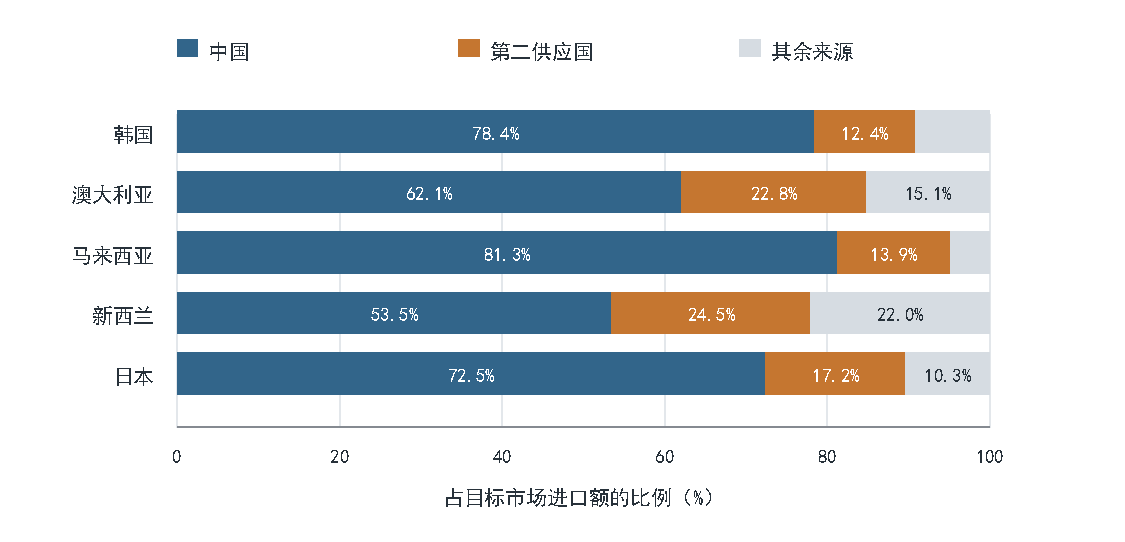
\includegraphics[width=0.84\textwidth]{supplier_concentration.pdf}
\caption{五个重点市场的供应来源结构}
\label{fig:supplier}
\begin{minipage}{0.84\textwidth}\small
数据来源：ITC Trade Map五国2025年按供应国进口派生表；按中国、第二供应国及其余来源分组。
\end{minipage}
\end{figure}

图\ref{fig:supplier}显示，中国在五国均占过半供应份额，但澳大利亚和新西兰的其他来源空间更大；日本、澳大利亚和新西兰的第二供应国均为马来西亚。结合第一部分所述区域制造布局，这一结构说明中国企业已具备稳定供给位置，同时开始利用RCEP区域生产网络。后续比较转向品牌、产品配置和价格带。

品牌层面，开源证券转引的2024年石头科技份额在韩国为30\%、澳大利亚为25\%。两国已有品牌基础，后续重点是以合适的产品和价格段扩大用户覆盖；日本则从产品层级和渠道表现继续识别品牌位置。\src{开源证券，2026年2月4日公司深度报告，第28页图43及正文，转引欧睿，采用2024年统计值。}

研报图43列示石头在马来西亚的2024年份额为8\%。开源证券认为消费者教育和价格带上移有助于中国品牌在东南亚深化经营；当地产品与报价将用于检验石头能否把这一趋势转化为品牌覆盖。\src{开源证券，2026年2月4日公司深度报告，第29页图43、第28页正文，转引欧睿。}

\begin{table}[H]
\centering
\caption{五国零售资料中已采得的五品牌扫地机产品页}
\label{tab:retailsample}
\small
\setlength{\tabcolsep}{4pt}
\begin{tabular}{lrrrrr}
\toprule
品牌 & 日本 & 韩国 & 澳大利亚 & 马来西亚 & 新西兰\\
 & Kakaku & Danawa & GetPrice & PriceShop & PriceSpy\\
\midrule
Roborock & 20 & 20 & 7 & 12 & 9\\
Ecovacs & 16 & 16 & 8 & 13 & 8\\
Xiaomi & 6 & 9 & --- & 13 & 6\\
Dreame & 13 & 19 & 4 & 6 & 12\\
Narwal & 8 & 10 & --- & --- & 2\\
\midrule
合计 & 63 & 74 & 19 & 44 & 37\\
\bottomrule
\end{tabular}
\par\vspace{0.4em}
\begin{minipage}{0.94\textwidth}\small
数据来源：Kakaku、Danawa、GetPrice、PriceShop与PriceSpy。韩国样本排除海外购；“---”表示未取得可读产品页。\src{価格.com（Kakaku，\url{https://kakaku.com/}）、Danawa（\url{https://www.danawa.com/}）、GetPrice（\url{https://www.getprice.com.au/}）、PriceShop（提供者Price Guide Sdn Bhd，\url{https://my.priceshop.com/en/}）与PriceSpy（\url{https://pricespy.co.nz/}）。}
\end{minipage}
\end{table}

日韩样本覆盖五个中国品牌，澳大利亚现有三品牌样本以逐型号观察为主。马来西亚四品牌取得产品页，云鲸另有上市和开店报道；新西兰石头、科沃斯、小米和追觅分别有8、5、6、7个有价产品。中国企业已在五国形成不同层次的产品布局，石头的适配重点相应落到配置、供货和保修。\src{PriceShop，2025年9月29日云鲸上市报道及2026年5月8日Sunway Velocity门店报道，\url{https://my.priceshop.com/en/news/narwal-freo-flow-freo-x10-pro-and-s30-malaysia/}、\url{https://my.priceshop.com/en/news/narwal-first-flagship-store-sunway-velocity-malaysia/}；来源ID为SRC-20261010-MYS-PriceShop-Narwal-20250929及SRC-20261010-MYS-PS-NEWS-narwal-store-20260508。}

竞争资料进一步区分了五国：韩国和澳大利亚是在既有品牌基础上深化，日本侧重产品层级与渠道验证，马来西亚要把中国供给优势转化为品牌覆盖，新西兰则围绕有限型号形成稳定服务。
% TODO[RETAIL-MY-NZ]: 更新PriceShop正常报价及缓存时点；补充两国授权分销、本地保修和同型号配置，继续区分型号、套装与地区变体。

\subsection{目标市场季节性分析}

石头科技年报指出，电商促销会带来销售波动，旺季需要协调采购、生产、仓储、配送和售后。季节性分析因此把促销排期、终端订单和履约能力放在同一时间轴上。\src{北京石头世纪科技股份有限公司，《2025年年度报告》，第48页，“销售季节性风险”。}

促销案例显示了不同市场的销售弹性。开源证券列示的2025年Black Friday期间，日本石头扫地机销量同比增长55\%；澳大利亚全渠道销量3.6万台，同比增长96\%，其中Amazon销量同比增长355\%。另据2024年10月研报转引公司战报，2024年7月Prime Day期间澳大利亚Amazon销量同比增长270\%。这些窗口数据适合用于安排备货和渠道资源，韩国则需从当地促销排期建立同类记录。\src{开源证券，2026年2月4日公司深度报告，第27页，2025年黑五公司销售表现；开源证券，《收入错期、费用前置下业绩阶段性承压，看好2024Q4内外销实现高增》，2024年10月31日，第1页，转引公司战报。}

澳大利亚两次促销案例都出现较大销量增幅，研究重点应从“旺季是否存在”进一步转向促销价、备货和售后能否承接集中订单；日本则要观察促销带来的新客是否转化为常态销售。韩国可先跟踪当地渠道的促销排期，再与订单、维修和退货记录匹配，不套用另外两国的峰值。

马来西亚有年末电商与门店活动两类线索。PriceShop列示2025年12.12小米S40从1,099降至699林吉特，折让36.4\%；云鲸在2026年5月8日开店当天赠送洗地机。中国品牌在当地同时使用折让、赠品和平台活动，石头可据此区分活动价与常态价，安排分层促销。\src{PriceShop，Raymond Saw，2025年12月9日12.12活动报道，\url{https://my.priceshop.com/en/news/xiaomi-malaysia-12-12-2025-sales-discount-promo/}；Hamka Rosli，2026年5月8日云鲸Sunway Velocity门店报道，\url{https://my.priceshop.com/en/news/narwal-first-flagship-store-sunway-velocity-malaysia/}；来源ID为SRC-20261010-MYS-PS-NEWS-xiaomi-1212-20251209及SRC-20261010-MYS-PS-NEWS-narwal-store-20260508，折让按(1099-699)/1099计算。}

新西兰35个产品页提供三个月价格摘要，26个有价型号中13个只有一条合格报价。现阶段先连续跟踪价格、库存和到货节奏，再据完整序列安排促销备货。\src{PriceSpy页面公开摘要；覆盖分母为37个产品页。}

季节性证据把市场增长进一步落实到经营节奏：日本关注促销后的新客留存，澳大利亚关注集中订单的履约与盈利，马来西亚区分多种促销工具，韩国和新西兰先完善本地时间序列。价格分析据此分别考察活动价、常态价和可交付价。

% TODO[RETAIL-SEASON]: 补充五国月度销售、搜索或零售数据；马来西亚在已有活动日期上补订单，新西兰在三个月公开价格摘要基础上建立完整序列，检验峰值及备货提前期。

\subsection{价格定位分析}

公司年报提出海外全价格段覆盖，零售快照也显示五个中国品牌正在形成各自的产品梯度。日本Roborock样本代表价从25,800日元至201,300日元，中位价94,390日元，高于其余四品牌；韩国中位价1,277,500韩元，高于科沃斯、小米和追觅，低于云鲸。石头在两国以中高价位为主，同时以较低价产品承接不同预算。\src{北京石头世纪科技股份有限公司，《2025年年度报告》，第20--22页；Kakaku、Danawa产品数据。Roborock日本最低、最高价格记录来源ID分别为SRC-0014、SRC-0024。}

\begin{figure}[H]
\centering
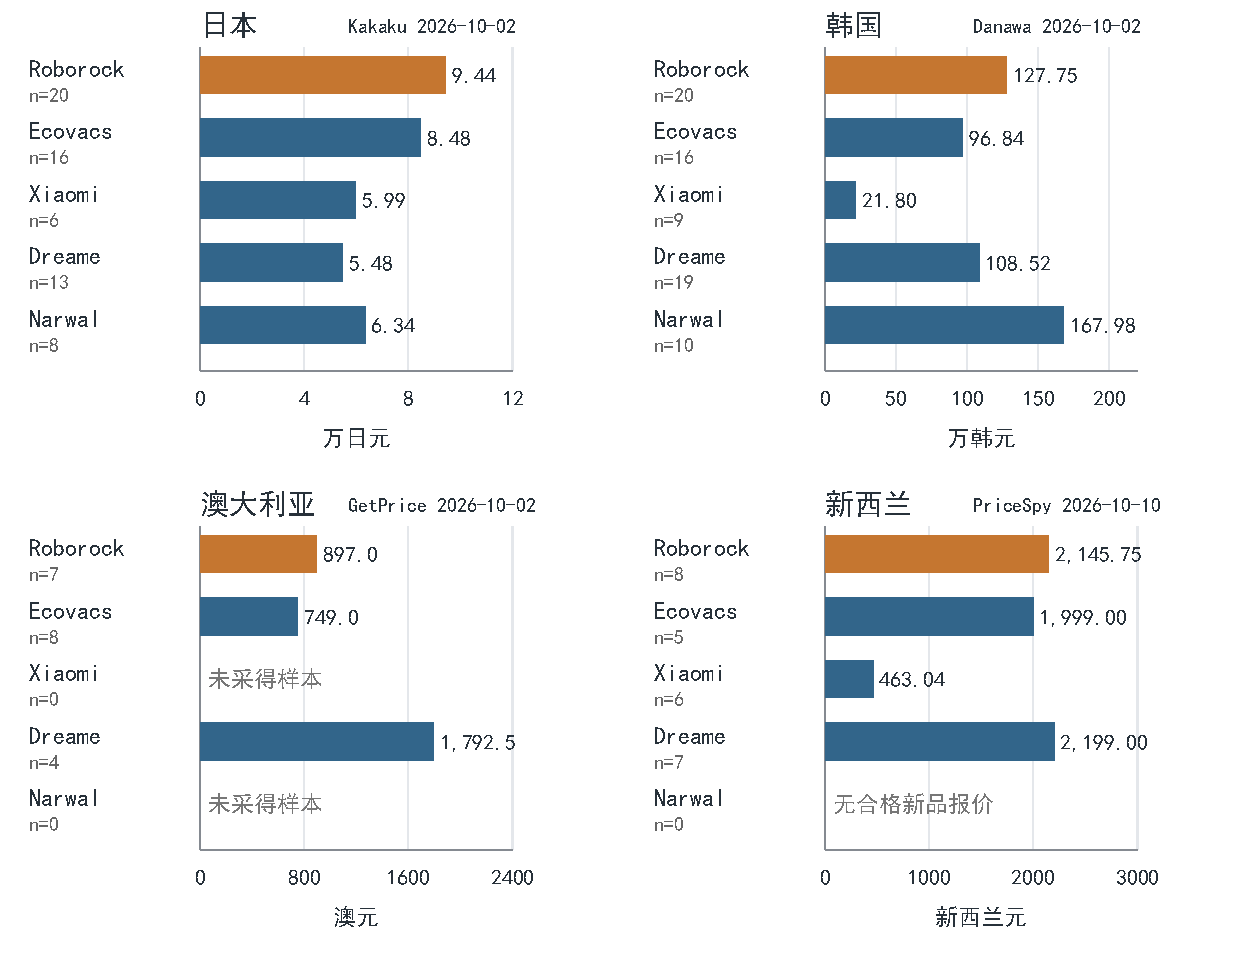
\includegraphics[width=\textwidth]{retail_brand_price_comparison.pdf}
\caption{日本、韩国、澳大利亚与新西兰零售快照的品牌代表价中位数}
\label{fig:retailprice}
\begin{minipage}{0.96\textwidth}\small
数据来源：Kakaku、Danawa、GetPrice与PriceSpy。日韩澳按正常报价中位数或最低正常报价形成产品代表价，新西兰按合格新品报价形成代表价；各面板再按品牌汇总，$n$为有价产品数。\src{日韩澳新西兰四国入图数分别为63、74、19、26条；韩国排除14条海外购。}
\end{minipage}
\end{figure}

澳大利亚样本中，石头中位价为897澳元，科沃斯为749澳元，追觅为1,792.5澳元。石头7条记录中有2条取得至少3家正常报价，以这2条计算的中位价为2,898.5澳元。中国品牌的价格梯度已经出现，石头在当地的定位应落实到具体型号、正常报价和供货状态。\src{GetPrice，Roborock来源ID为SRC-AUS-0003至SRC-AUS-0009；至少3条正常报价的记录为Saros 20（代表价2,999澳元）与Qrevo Edge 2 Pro（2,798澳元）。本研究据normal\_offer\_count字段筛选并计算。}

新西兰的中国品牌样本已覆盖多个价位，石头样本中位价接近追觅，高于科沃斯和小米，分布见表\ref{tab:nzlprice}。Q7B+、Qrevo 2 Pro与Saros 20代表价分别为499、1,893.50和3,265.50新西兰元，可沿这一型号梯度检验功能价差与购买理由。\src{PriceSpy品牌中位数按有合格新品报价的产品代表价计算。Q7B+、Qrevo 2 Pro及Saros 20页面分别为\url{https://pricespy.co.nz/product.php?p=16004718}、\url{https://pricespy.co.nz/product.php?p=16964950}、\url{https://pricespy.co.nz/product.php?p=16030637}；来源ID为SRC-20261010-NZL加对应产品ID。}

\begin{table}[H]
\centering
\caption{新西兰有价产品样本的品牌价格分布}
\label{tab:nzlprice}
\small
\begin{tabular}{lrrrr}
\toprule
品牌 & 有价产品数 & 最低代表价 & 代表价中位数 & 最高代表价\\
 & & \multicolumn{3}{c}{新西兰元}\\
\midrule
Roborock & 8 & 499.00 & 2,145.75 & 3,265.50\\
Ecovacs & 5 & 899.00 & 1,999.00 & 2,999.00\\
Xiaomi & 6 & 226.31 & 463.04 & 1,047.59\\
Dreame & 7 & 888.00 & 2,199.00 & 3,296.00\\
Narwal & 0 & --- & --- & ---\\
\bottomrule
\end{tabular}
\par\vspace{0.4em}
\begin{minipage}{0.94\textwidth}\small
数据来源：PriceSpy公开页面。价格按26个有价型号分别计算后汇总；产品页总数见表\ref{tab:retailsample}。
\end{minipage}
\end{table}

库存条件会改变价格判断。Qrevo C Pro两条报价为899和1,885.25新西兰元，中位数1,392.13元；低价库存未知，仅留在库报价时升至1,885.25元。定位须同时核对可交付价格与保修。\src{PriceSpy，Roborock Qrevo C Pro，\url{https://pricespy.co.nz/product.php?p=15953163}来源ID SRC-20261010-NZL-15953163。Farmers报价899元，页面标注Unknown stock；Ascent报价1,885.25元，页面标注In stock。}

马来西亚以PriceShop新品报道识别梯度：2026年5月20日Qrevo S Pro与Curv 2 Flow分别为2,699和3,999林吉特，5月19日Saros 20为5,399林吉特。三个价位为功能分层提供了基础，下一步检验减少维护等功能能否支持价差。\src{PriceShop（Price Guide Sdn Bhd），Raymond Saw，2026年5月20日Qrevo系列报道，\url{https://my.priceshop.com/en/news/roborock-qrevo-curv-2-flow-and-qrevo-s-pro-powerful-everyday-robot-vacuums-from-rm2699/}；2026年5月19日Saros 20系列报道，\url{https://my.priceshop.com/en/news/roborock-saros-20-series-their-most-advanced-premium-robot-vacuums-yet-from-rm5399/}；来源ID为SRC-20261010-MYS-PS-NEWS-roborock-qrevo-20260520及SRC-20261010-MYS-PS-NEWS-roborock-saros-20260519。}

最终零售价应从目标贡献毛利倒推：

\begin{equation}
P=\frac{C_{FOB}+C_{freight}+C_{duty}+C_{channel}+C_{service}}{1-m},
\end{equation}

其中$m$为目标贡献毛利率，服务成本包括退换货、维修、备件和客服。各国、各型号据实际渠道和服务条件分别设定$m$，由此检验零售价格对经营成本的覆盖程度。

价格证据最终形成五项任务：日本和韩国验证中高价功能的说服力，澳大利亚检验促销后的正常报价与盈利，马来西亚检验产品梯度，新西兰检验可交付价格对服务成本的覆盖。第五部分至此完成从市场机会到经营问题的转换。

% TODO[RETAIL-SKU]: 补充澳大利亚小米与云鲸样本，增加正常报价覆盖，并按同档功能、上市时间和本地保修条件作逐型号比较。
% TODO[WIND-PRODUCT]: 补充五国分价格带整机收入、销量与ASP，并与当地SKU正常报价匹配。

\section{前景分析}

\subsection{五国市场机会与石头科技适配}

第五部分已将五国机会转化为不同的经营问题。本节不再重复排名，而是把这些问题分别落实到产品、价格、渠道服务和合规安排。

欧美案例说明石头已经具备自有品牌经营、产品分层和渠道扩展能力。将这一能力用于RCEP时，日本侧重解释升级价值，韩国理顺代理商的营销和服务职责，澳大利亚检验促销后的常态盈利；马来西亚沿已有产品梯度扩大体验与服务触点，新西兰围绕少量核心型号衔接当地零售商。

\subsection{产品}

高端产品与较低价系列并行，早已出现在石头的外销布局中。开源证券2022年报告记录，S7 MaxV Ultra定价1,399美元，同时布局Q系列。该案例说明公司具有以功能分层覆盖不同预算的经验，五国选品可沿旗舰、中端和基础功能三个层级展开。\src{开源证券，《Q2内销高增、美亚逆势增长，费用投放效率提升》，2022年9月1日，第1页“外销方面”，1,399美元为该报告记录的历史外销定价。}

官网产品矩阵可把适配问题落到具体功能。Saros 10R具有7.98厘米机身和底盘升降，适合检验低矮家具与门槛通过；Qrevo 2 Pro配置地毯自动卸拖布和防缠绕结构，可检验混合地面、毛发清理与日常维护；Q10系列提供自动集尘、激光导航和避障，构成较低门槛的功能组合。进入五国时，再以当地在售配置连接具体居住场景。\src{Roborock官方产品页：Saros 10R（\url{https://us.roborock.com/pages/roborock-saros-10r}）、Qrevo 2 Pro（\url{https://us.roborock.com/pages/roborock-qrevo-2-pro}）、Q10 Series（\url{https://global.roborock.com/pages/roborock-q-series}）。}

日本零售样本已经包含Q7、Qrevo和Saros等层级，可比较不同配置对价差的支撑；韩国结合较宽的卖家覆盖，比较全能基站款的功能和服务承诺；澳大利亚则把地毯处理、防缠绕与售后备件列为实测项目。中国品牌早期出海曾出现产品卖点与海外地毯清扫需求错配的情况，这一经验要求五国选品从当地家庭的清洁问题出发。\src{Kakaku、Danawa产品样本；开源证券，2026年2月4日公司深度报告，第13页。}

马来西亚沿Qrevo、Saros梯度检验减少维护能否支持升级。新西兰围绕少量型号比较功能：PriceSpy的Qrevo C Pro列有激光导航、自动集尘和拖布烘干，Saros 20还列有障碍感知，可据此连接配置、体验与价格。\src{马来西亚产品梯度见第5.4节PriceShop新品报道。PriceSpy，Roborock Qrevo C Pro与Saros 20，\url{https://pricespy.co.nz/product.php?p=15953163}、\url{https://pricespy.co.nz/product.php?p=16030637}；来源ID为SRC-20261010-NZL-15953163及SRC-20261010-NZL-16030637。}

\subsection{价格}

价格判断与第5.4节衔接：日本与韩国样本支持中高价位产品覆盖，澳大利亚需要补足逐型号正常报价；马来西亚区分新品报道价与活动价，新西兰区分有价产品与可交付报价。第3.2节已经显示，公司销量和收入扩张伴随毛利率、净利率与经营现金净流量下降。2025年境外主营业务毛利率为48.15\%，较上年下降5.55个百分点；直营收入89.73亿元，同比增长71.20\%，直营毛利率下降7.41个百分点。结合中国头部企业的降本经验，五国选品应把促销折让、物料成本与单台服务负担纳入同一张贡献表。\src{北京石头世纪科技股份有限公司，《2025年年度报告》，第54--55页，分地区、分销售模式收入成本表及变动原因说明。直营收入原值8,972,779,823元；中国头部企业成本管理经验见第3.2节。}

日本检验升级功能能否支持价差，韩国把代理责任与价格纪律一并考察，澳大利亚检验促销后的常态售价和单台贡献。马来西亚将优惠原产条件、赠品和正常售价纳入测算；新西兰在扩充SKU前核对单台物流、维修和备件负担。五国均按第5.4节的成本关系检验售价。

美国样本说明，公司已有按渠道区分型号和折扣的实践。开源证券2026年2月报告表3列示，Target的Q10 PF+销售价为319.99美元，渠道特供款为399.99美元；Qrevo Curve的列示价与销售价分别为1,599.99和799.99美元。用于五国时，应把实际售价、渠道型号和保修条件一并比较。\src{开源证券，《公司深度报告：新业务大幅减亏+扫地机行业竞争缓和，2026年净利率迎来拐点》，2026年2月4日，第21页表3。}

\subsection{人员、渠道与服务}

日本与韩国已有海外公司，本地经营可以沿既有组织补足用户反馈、维修与备件协同。开源证券2026年9月报告称，韩国采用FSD（Full-Service Distributed）代理模式，相关费用主要由代理商投放。韩国开拓的重点是明确代理商的营销和服务职责、客户数据回流方式，以及不同卖家的价格管理。\src{北京石头世纪科技股份有限公司，《2022年年度报告》，第12页；开源证券，《降本提效叠加竞争格局改善，扫地机龙头有望迎来业绩收获期》，封面日期2026年9月6日，第17页“亚太”。}

多品牌经营和渠道间价格差异会影响合作伙伴投入。日本的多层级产品、韩国的代理合作和澳大利亚的促销供货，都需要明确型号分工、价格沟通、当地语言客服与退换修责任。服务网络与渠道同步推进，并以退货率、维修周期和备件可得性评价经营质量。\src{北京石头世纪科技股份有限公司，《2025年年度报告》，第49--50页，海外经营与经销商管理风险。}

欧洲经验还涉及渠道切换的回收节奏。开源证券将2024年第三季度欧洲阶段性承压解释为渠道结构调整下经销收入延后确认，同时称线上增长良好。五国深化渠道时，应分别跟踪终端销售、经销商库存与公司回款，以此衡量门店扩展的经营效果。\src{开源证券，《收入错期、费用前置下业绩阶段性承压，看好2024Q4内外销实现高增》，2024年10月31日，第1页“欧洲”。}

中国品牌在马来西亚已形成线上线下结合的渠道实践。PriceShop的2025年云鲸上市报道列有官方Shopee店及Aihome门店，2026年又报道Sunway Velocity品牌店。石头可据这些本地触点设计演示、线上转化和售后的伙伴分工，并与当地代工形成供应协同。\src{PriceShop，2025年9月29日云鲸上市报道及2026年5月8日Sunway Velocity门店报道；来源ID为SRC-20261010-MYS-PriceShop-Narwal-20250929及SRC-20261010-MYS-PS-NEWS-narwal-store-20260508。}

新西兰Saros 20页面列出Farmers、Heathcote Appliances、JB Hi-Fi和Ascent，后三家标注在库。可从这些零售触点核实授权、退换修与备件责任，形成少量核心型号持续销售的渠道基础。\src{PriceSpy，Roborock Saros 20，\url{https://pricespy.co.nz/product.php?p=16030637}；来源ID为SRC-20261010-NZL-16030637。}

五国渠道安排虽有差异，判断标准是一致的：合作责任清晰、终端销售能够转为回款、服务网络能够承接退换修。达到这些条件后，再扩大SKU和零售触点。

\subsection{许可、合规与RCEP规则}

上市前应核对目的国的电器安全、无线通信、能效和消费者保护要求。RCEP规则进一步影响关税适用、原产资格、证明文件和通关流程。

RCEP第2.4条要求成员方对原产货物按附件一承诺表实施关税减让；当实际最惠国税率更低时，进口商可以适用更低的最惠国税率。第2.6条处理不同出口方税率存在差异时的“RCEP原产国”问题，第2.7条和第2.14条要求以协调制度归类并处理税表转版。企业需要先映射进口国税则线，再判断原产资格，最后比较可用方案。表\ref{tab:rceptariff}按更新后的ITC记录区分MFN、RCEP与其他对华优惠。\src{《区域全面经济伙伴关系协定》第2章“货物贸易”，第2.4、2.6、2.7和2.14条。}

\begin{table}[H]
\centering
\caption{五个重点市场HS850811相关税则线的关税记录（2026年）}
\label{tab:rceptariff}
\small
\begin{tabular}{p{2.0cm}p{3.4cm}rrp{3.8cm}}
\toprule
市场 & 税则线 & MFN & RCEP & 其他对华优惠\\
\midrule
韩国 & 8508111000\newline（机器人型） & 8\% & 5.30\% & 0\%（另列对华方案）\\
澳大利亚 & 85081100 & 0\% & 未单列 & 未单列\\
马来西亚 & 8508110000 & 20\% & 18.20\% & 0\%（另列对华方案）\\
新西兰 & 85081100 & 0\% & 未单列 & 未单列\\
日本 & 850811010\newline850811090 & 0\% & 未单列 & 未单列\\
\bottomrule
\end{tabular}
\par\vspace{0.4em}
\begin{minipage}{0.92\textwidth}\small
资料来源：ITC Market Access Map，税率年份2026，HS Rev.2022；“未单列”表示返回结果中未列该方案。\src{ITC Market Access Map；来源ID为MACMAP-410-DUTY-8508111000、MACMAP-036-DUTY-85081100、MACMAP-458-DUTY-8508110000、MACMAP-554-DUTY-85081100、MACMAP-392-DUTY-850811010及850811090。}
\end{minipage}
\end{table}

日本、澳大利亚和新西兰的MFN已为零，关税对三国排序影响较小；韩国和马来西亚需比较RCEP与其他对华优惠，并将税率和原产证明成本纳入第5.4节的单台贡献测算。

取得RCEP优惠待遇的前提落在第3章。第3.2条规定原产货物的基本类型；HS2022产品特定原产地规则对8508.11给出“CTSH或RVC40”两条可选路径：非原产材料发生六位子目改变，或者区域价值成分达到40\%。\src{《区域全面经济伙伴关系协定》第3章第3.2条；RCEP秘书处《产品特定原产地规则（HS2022）》，2022年8月20日编辑修订，第118页8508.11行。} CTSH核对BOM中非原产零部件与整机的六位子目关系，RVC40保存FOB价值、非原产材料价值和计算底稿。若改用其他协定的优惠税率，应另按该协定的原产地规则核验。

第3.4条允许区域累积：来自其他RCEP成员方的原产材料用于中国生产时，可按规则视为中国生产中的原产材料。\src{《区域全面经济伙伴关系协定》第3章“原产地规则”，第3.4条“累积”。} 这对电机、传感器、芯片、电池或其他区域采购件具有直接意义。第一部分所述越南、马来西亚代工与区域采购，只有在BOM、加工过程和证明文件满足原产规则时，才能进一步形成关税与交付优势。

第3.6条排除仅包装、简单装配等微小加工，第3.7条允许在规定限度内处理未满足税则归类改变的少量非原产材料，第3.15条要求经第三方运输时保持海关监管并限制额外加工。第3.16至3.18条规定原产地证明方式和最低信息，第3.27条要求保存相关记录。\src{《区域全面经济伙伴关系协定》第3章第3.6、3.7、3.15、3.16--3.18和3.27条；《中华人民共和国海关〈区域全面经济伙伴关系协定〉项下进出口货物原产地管理办法》，海关总署令第255号。}

这些条款可转化为一套出口证据链：产品型号对应进口国税则线，BOM对应CTSH或RVC40计算，供应商声明支持区域累积，商业发票与原产地证明保持一致，提单和中转记录支持直接运输。证据链在首批出货前完成，后续每次BOM或供应商变化都触发原产资格复核。

RCEP第4章的预裁定、风险管理和货物放行条款可以降低通关不确定性；第6章对标准、技术法规和合格评定提出透明度与合作框架。扫地机仍要完成目的国的电器安全、电磁兼容、无线模块、电池和标签要求，但企业可以通过预裁定和提前提交完整技术文件减少归类与放行反复。\src{《区域全面经济伙伴关系协定》第4章“海关程序和贸易便利化”及第6章“标准、技术法规和合格评定程序”。}

\subsection{差异化前景判断}

韩国拥有较大的进口规模和既有品牌基础，适合深化代理服务，以职责、回款和售后指标推动增长承接。澳大利亚规模与增速兼具，促销弹性也较强，开拓重点是把旺季销量转化为常态销售和单台贡献。日本保留最大的需求池，应以多层级产品解释替代与升级价值。马来西亚增长较快且已有产品梯度，可通过价格分层、体验触点和区域供应协同扩大品牌覆盖。新西兰相对潜力较高而绝对容量有限，宜以少量核心型号连接零售商，控制备货和维修负担。

公司收入扩张伴随毛利率、净利率和经营现金净流量下降，五国开拓因而以需求转化、单台贡献和回款质量作为共同门槛。各国先通过相应门槛，再扩大SKU与渠道。

\section{结论}

全文形成了一条由供给到经营的分析链：中国产品开发和区域供给能力构成开拓基础，中国在重点市场已有稳定供应位置，五国名单经产品口径检验仍保持稳定；终端资料进一步把机会分解为增长承接、常态盈利、存量升级、品牌覆盖和轻量经营五项任务。

石头在欧美积累的自有品牌、多层级产品和本土渠道经验，为五国执行提供了能力基础。RCEP开拓应按成熟市场深化、增长市场转化和小市场轻量验证的次序推进，并以单台贡献、回款和服务质量决定扩张节奏。

\begin{table}[H]
\centering
\caption{阶段性市场开拓方向}
\label{tab:roadmap}
\small
\begin{tabular}{p{2.0cm}p{3.6cm}p{5.1cm}p{3.1cm}}
\toprule
阶段 & 时间与任务 & 主要交付 & 决策指标\\
\midrule
准备期 & 第1季度：核对五国归类、认证、渠道与售后 & 分国核心SKU和备件；马来西亚价格及促销条件；新西兰可交付报价与保修 & 合规完成率、到岸成本、服务覆盖\\
试销期 & 第2季度至第3季度：按本地排期开展渠道验证 & 韩国核对代理职责与回款；日本验证升级转化；澳大利亚验证促销后常态盈利；马来西亚检验分价格带转化；新西兰检验少量型号供货与退换修 & 转化率、退货率、维修周期、单台贡献毛利\\
扩张期 & 第4季度后：分国旺季与年度复盘 & 比较促销后常态销售、库存和服务负担，再判断SKU与渠道扩充 & 获客成本、耗材复购、库存周转、回款周期\\
\bottomrule
\end{tabular}
\par\vspace{0.4em}
\begin{minipage}{0.92\textwidth}\small
资料来源：本研究依据ITC筛选结果、企业年报季节性信息与RCEP原产地规则设计。
\end{minipage}
\end{table}


\begingroup
\sloppy
\theendnotes
\endgroup

\end{document}
